\documentclass[tcc, capa, capa-completa, english]{ufxc}

% capa: imprime a parte da frente da capa em uma única página
% capa-completa: imprime a versão completa da capa, com a parte da frente, verso, lombada e as orelhas

% =====================================================
% Pacotes usados no projeto
% =====================================================

\usepackage[style=abnt, noslsn]{biblatex} %, language=brazil
\usepackage{tocloft}
\let\printglossary\relax
\let\theglossary\relax
\let\endtheglossary\relax

% \usepackage[brazilian,hyperpageref]{backref}   % Paginas com as citações na bibl
% \usepackage[alf]{abntex2cite} % Citações padrão ABNT

\usepackage[noredefwarn, acronyms, symbols]{glossaries}
\usepackage[lined,boxed,ruled,commentsnumbered]{algorithm2e}


% \usepackage{pgf}
% \usepackage{tikz}
% \usepackage{hhline}
% \usepackage{xfrac}
% \usepackage[export]{adjustbox} % http://tex.stackexchange.com/questions/163246/resize-a-tabular-object-to-textwidth
% \usepackage{rotating}
% \usepackage{pdflscape}
% \usepackage{amsmath}
% \usepackage{amstext}
% \usepackage{amsfonts}
% \usepackage{amssymb}
% \usepackage{mathtools}
% \usepackage{amsthm}
% \let\openbox\relax
% \usepackage{bm}

% % \DeclarePairedDelimiter\floor{\lfloor}{\rfloor}
% \usepackage[makeroom]{cancel}
% \usepackage{color}    % Possibilita o uso de cores no documento
% \usepackage{colortbl}
\usepackage{subfig} % Usado para separar figuras em sub-figuras (ambiente subfloat) 
% \usepackage{scalefnt}
\usepackage{multirow}
% \usepackage{iflang} %there is a warning which will be corrected in future texmf dist.
% \usepackage[lined,boxed,ruled,commentsnumbered]{algorithm2e}
% \usepackage{soul}

% \usepackage{xspace} %In init/math

\usepackage{todonotes}
\usepackage{tabularx}
\usepackage{pgfgantt}

% Code Snippets
\usepackage{listings}
\renewcommand{\lstlistingname}{Código}
\lstset{
    basicstyle=\scriptsize\ttfamily,
	numbers=left,
	stepnumber=1,
	numbersep=-0.5em,
	keywordstyle=\color{blue},
	commentstyle=\color{black},
	stringstyle=\color{black},
    numberstyle=\scriptsize\ttfamily\color{black},
	frame=single,
	tabsize=2,
	float,
	language=C++,
	captionpos=t,
	showstringspaces=false,
	backgroundcolor=\color{white},
	morekeywords = {Array2D, __parallel__, Mask2D, Stencil2D},
	emph={
		pragma,
		omp,
		parallel,
		reduction,
		schedule,
		private,
		shared
	},
	emphstyle={\color{blue}}%
}

% =====================================================
% Local/data
% =====================================================

\local{Florianópolis}
\data{01}{Junho}{2019}

% =====================================================
% Informações do programa
% =====================================================

\instituicao{Universidade Federal de Santa Catarina}
\centro{Centro Tecnológico}
\departamento{Departamento de Informática e Estatística}
\grau{bacharel}
\curso{Ciência da Computação}
\coordenador{Nome do Coordenador do Curso}

% =====================================================
% Título e Informações sobre o autor
% =====================================================

\titulo{A Inter-Cluster Communication Module of a Hardware Abstraction Layer for Lightweight Manycore Processors}
% \subtitulo{}

\autor{João Vicente}{Souto}

%formato para orientador e coorientador:
%\orientador[genero]{titulação}{primeiros nomes}{sobrenome}{Universidade}
\orientador{Dr.}{Márcio Bastos}{Castro}{Universidade Federal de Santa Catarina}
\coorientador{Me.}{Pedro Henrique}{Penna}{Université Grenoble Alpes}

% =====================================================
% informações da banca
% =====================================================
% * assume-se que o orientador é parte da banca avaliadora
\coorientadorNaBanca{}

%formato para membro da banca
%\membroBanca{Nome}{Afiliação}
\membroBanca{Prof$^a$. Dr$^a$. Membro A. First}{Universidade Federal de Santa Catarina}
\membroBanca{Prof. Dr. Membro B.}{Universidade Federal de Santa Catarina}
\membroBanca[video]{Prof. Dr. Membro C.}{Universidade Federal de Santa Catarina}


% =====================================================
% Informações do trabalho
% =====================================================

%as palavras-chave devem ser definidas antes do início do documento pois
%a capa e também a lista catalográfica dependem delas...
% \palavrasChave{{latex},{abntex},{editoração de texto}}
%perceba a maneira como cada palavra chave é definida. Tal modo deve ser 
%mantido para a correta geração da ficha catalográfica

% por algum motivo ainda não identificado, ocorre um erro se os dois não forem definidos e as palavras não são impressas na ficha catalográfica
\palavrasChave{{Template}, {Ufsc}, {Latex}, {BU}}
\palavrasChave[english]{{Template}, {Ufsc}, {Latex}, {BU}}

% ---
% compila o indice
% ---
\makeindex
% ---

% {glossaries} package
% \makeglossaries
% \loadglsentries{init/acronyms}
% \loadglsentries{init/symbols}
\glsdisablehyper

%%%%%%%%%%%%%%%%%%%%%%%%%%%%%%%%%%%%%%%%%%%%%%%%%%%%%%%%%%%%%%%%%%%%
%%% Acronyms list                                                %%%
%%%%%%%%%%%%%%%%%%%%%%%%%%%%%%%%%%%%%%%%%%%%%%%%%%%%%%%%%%%%%%%%%%%%
%%% Importante:                                      
%%% - A lista PRECISA SER MANTIDA ORDENADA
%%%%%%%%%%%%%%%%%%%%%%%%%%%%%%%%%%%%%%%%%%%%%%%%%%%%%%%%%%%%%%%%%%%%

%A
\xnewacronym[amp]{AMP}{Asymmetric Multi-Processing}
\xnewacronym[anova]{ANOVA}{Analysis of Variance}
\xnewacronym[api]{API}{Application Programming Interface}

%B

%C
\xnewacronym[cnoc]{C-NoC}{Control Network-on-Chip}
\xnewacronym[cmp]{CMP}{Chip Multiprocessor}
\xnewacronym[cow]{COW}{Copy-On-Write}
\xnewacronym[cpu]{CPU}{Central Processing Unit}

%D
\xnewacronym[dnoc]{D-NoC}{Data Network-on-Chip}
\xnewacronym[dma][longplural={Direct Memory Accesses}]{DMA}{Direct Memory Access}
\xnewacronym[dram][longplural={Dynamic Random Access Memories}]{DRAM}{Dynamic Random Access Memory}
\xnewacronym[dtlb]{DTLB}{Data Translation Lookaside Buffer}

%E

%F
\xnewacronym[flops]{FLOPS}{\textit{Floating-point Operations per Second}}
\xnewacronym[fos]{FOS}{Factored Operating System}
\xnewacronym[fpga]{FPGA}{Field Programmable Gate Array}

%G
\xnewacronym[gpu]{GPU}{Graphics Processing Unit}

%H
\xnewacronym[hal]{HAL}{Hardware Abstraction Layer}
\xnewacronym[hpc]{HPC}{High-Performance Computing}

%I
\xnewacronym[iid]{i.i.d}{Independent and Identically Distributed}
\xnewacronym[ipc]{IPC}{Inter-Process Communication}
\xnewacronym[isa]{ISA}{Distributed Hash Table}
\xnewacronym[itlb]{ITLB}{Instruction Translation Lookaside Buffer}
\xnewacronym[ieee]{IEEE}{Institute of Electrical and Electronics Engineers}

%J
\xnewacronym[jtlb]{JTLB}{Join Translation Lookaside Buffer}

%K

%L
\xnewacronym[lfour]{L4}{L4 Microkernel}
\xnewacronym[ltlb]{LTLB}{Locked Translation Lookaside Buffer}

%M
\xnewacronym[mimd]{MIMD}{Multiple Instruction Multiple Data}
\xnewacronym[misd]{MISD}{Multiple Instruction Single Data}
\xnewacronym[mmio]{MMIO}{Memory-Mapped I/O}
\xnewacronym[mmu]{MMU}{Memory Management Unit}
\xnewacronym[moosca]{MOOSCA}{Manycore Operating System for Safety-Critical Application}
\xnewacronym[mos]{mOS}{multi Operating System}
\xnewacronym[mpsoc]{MPSoC}{Multiprocessor System-on-Chip}
\xnewacronym[mpu]{MPU}{Memory Protection Unit}

%N
\xnewacronym[noc]{NoC}{Network-on-Chip}
\xnewacronym[norma]{NoRMA}{No Remote Memory Access}
\xnewacronym[nos]{nOS}{Nano-Sized Operating System}
\xnewacronym[numa]{NUMA}{Non-Uniform Memory Access}

%O
\xnewacronym[os]{OS}{Operating System}

%P
\xnewacronym[pe]{PE}{Processing Element}
\xnewacronym[pgas]{PGAS}{Partitioned Global Address Space}
\xnewacronym[pmca]{PMCA}{Programmable Manycore Accelerator}
\xnewacronym[pmio]{PMIO}{Port-Mapped I/O}
\xnewacronym[posix]{POSIX}{Portable Operating System Interface}

%Q
\xnewacronym[qos]{QoS}{Quality of Service}

%R
\xnewacronym[rab]{RAB}{Remapping Address Block}
\xnewacronym[ram][longplural={Random Access Memories}]{RAM}{Random Access Memory}
\xnewacronym[risc]{RISC}{Reduced Instruction Set Computer}
\xnewacronym[rm]{RM}{Resource Manager}
\xnewacronym[rma][longplural={Remote Memory Accesses}]{RMA}{Remote Memory Access}
\xnewacronym[rmem][longplural={Remote Memories}]{RMem}{Remote Memory}

%S
\xnewacronym[simd]{SIMD}{Single Instruction Multiple Data}
\xnewacronym[sisd]{SISD}{Single Instruction Single Data}
\xnewacronym[shm]{SHM}{POSIX Shared Memory}
\xnewacronym[smp]{SMP}{Symmetric Multi-Processing}
\xnewacronym[soc]{SoC}{System-on-a-Chip}
\xnewacronym[spm][longplural={Software-managed Scratchpad Memories}]{SPM}{Software-managed Scratchpad Memory}
\xnewacronym[sram][longplural={Static Random Access Memories}]{SRAM}{Static Random Access Memory}
	
%T
\xnewacronym[tlb]{TLB}{Translation Lookaside Buffer}

%U
\xnewacronym[uma][longplural={Uniform Memory Accesses}]{UMA}{Uniform Memory Access}

%V
\xnewacronym[vliw]{VLIW}{Very Long Instruction Word}

%W
\xnewacronym[watts]{W}{\textit{Watts}}

%%% Local Variables:
%%% mode: latex
%%% TeX-master: "main"
%%% End:

%% List of Symbols

\newglossaryentry{jcost}%
{%
	name={\ensuremath{j_{\text{cost}}}},
	description={The lagrangian rate-distortion cost of selecting a given candidate as reference},
	sort={J},
	type=symbols
}

\newglossaryentry{jlambda}%
{%
	name={\ensuremath{\lambda}},
	description={The Lagrange multiplier.},
	sort={lambda},
	type=symbols
}

% numbers 

\newglossaryentry{naturalnumbers}%
{%
	name={\ensuremath{\mathbb{N}}},
	description={The set of natural numbers. },
	sort={Number Natural},
	type=symbols
}

\newglossaryentry{rationalnumbers}%
{%
	name={\ensuremath{\mathbb{Q}}},
	description={The set of rational numbers. },
	sort={Number Rational},
	type=symbols
}

\newglossaryentry{integernumbers}%
{%
	name={\ensuremath{\mathbb{Z}}},
	description={The set of integer numbers. },
	sort={Number Integer},
	type=symbols
}

\newglossaryentry{realnumbers}%
{%
	name={\ensuremath{\mathbb{R}}},
	description={The set of real numbers. },
	sort={Number Real},
	type=symbols
}


%\glsaddall
\usepackage{xspace}
\DeclareMathOperator*{\argmin}{arg\,min}

\newtheorem{theorem}{{Theorem}}
\newtheorem{property}{Property}

\newtheorem{definition}{Definition}
\newtheorem{lemma}{Lemma}[definition]

\DeclareMathAlphabet{\mathcal}{OMS}{cmsy}{m}{n}
\DeclareMathAlphabet{\mathbfcal}{OMS}{cmsy}{b}{n}




\newcommand\qedsymbol{$\blacksquare$} %renewcommand o

\makeatletter
\renewcommand*\env@matrix[1][*\c@MaxMatrixCols c]{%
  \hskip -\arraycolsep
  \let\@ifnextchar\new@ifnextchar
  \array{#1}}
\makeatother

\newcommand{\jcost}{\gls{jcost}\xspace}
\newcommand{\jlambda}{\gls{jlambda}\xspace}

\newcommand{\naturals}{\gls{naturalnumbers}}
\newcommand{\integers}{\gls{integernumbers}}
\newcommand{\reals}{\gls{realnumbers}}

\newcommand{\primes}{\ensuremath{\mathbb{P}}}
\newcommand{\rationals}{\ensuremath{\mathbb{Q}}}
\newcommand{\complex}{\ensuremath{\mathbb{C}}}
\newcommand{\quaternions}{\ensuremath{\mathbb{H}}}


\addbibresource{references.bib} % {biblatex} package
% \bibliography{references}

%%these will be used in the large cover
% \pequenoResumo{Esse é o pequeno resumo que vai aparecer na orelha orelha direita da capa.}
% \bairro{Trindade}
% \cidade{Florianópolis}
% \estado{SC}

% =====================================================
% Comandos do usuário
% =====================================================

\newcommand{\note}[1]{\textbf{\textcolor{blue}{\hl{#1}}}} % {color, soul} package

% adiciona automaticamente \centering em ambientes tipo float
\makeatletter
\g@addto@macro\@floatboxreset\centering
\makeatother

% Caso prefira referenciar acronimos com \ac e \acp.
% \newcommand{\ac}[1]{\gls{#1}}
% \newcommand{\acp}[1]{\glspl{#1}}

% =====================================================
% Início do documento
% =====================================================
\begin{document}

% Seleciona o idioma do documento (conforme pacotes do babel)
\selectlanguage{english}

% =====================================================
% Pré-textuais
% =====================================================

% \imprimircapa
\imprimirfolhaderosto* % (o * indica que haverá a ficha bibliográfica)

% \imprimirFichaCatalografica{} % pode passar pdf por parametro
% \begin{errata}
% Elemento opcional da \textcite[4.2.1.2]{liu08}. Exemplo:

\vspace{\onelineskip}

FERRIGNO, C. R. A. \textbf{Tratamento de neoplasias ósseas apendiculares com
reimplantação de enxerto ósseo autólogo autoclavado associado ao plasma
rico em plaquetas}: estudo crítico na cirurgia de preservação de membro em
cães. 2011. 128 f. Tese (Livre-Docência) - Faculdade de Medicina Veterinária e
Zootecnia, Universidade de São Paulo, São Paulo, 2011.

\begin{table}[htb]
\center
\footnotesize
\begin{tabular}{|p{1.4cm}|p{1cm}|p{3cm}|p{3cm}|}
  \hline
    \textbf{Folha} & \textbf{Linha}  & \textbf{Onde se lê}  & \textbf{Leia-se}  \\
    \hline
    1 & 10 & auto-conclavo & autoconclavo\\
    \hline
\end{tabular}
\end{table}

\end{errata}
% ---
% \inserirFolhaDeAprovacao{} % pode passar pdf por parametro

% \begin{dedicatoria}
  \vspace*{\fill}
  \centering
  \noindent
  \textit{ Este trabalho é dedicado às crianças adultas que,\\
  quando pequenas, sonharam em se tornar cientistas.} \vspace*{\fill}
\end{dedicatoria}
% % Agradecimentos
% ---
\begin{agradecimentos}
Os agradecimentos principais são direcionados à Gerald Weber, Miguel Frasson,
Leslie H. Watter, Bruno Parente Lima, Flávio de Vasconcellos Corrêa, Otavio Real
Salvador, Renato Machnievscz\footnote{Os nomes dos integrantes do primeiro
projeto abn\TeX\ foram extraídos de
\url{http://codigolivre.org.br/projects/abntex/}} e todos aqueles que
contribuíram para que a produção de trabalhos acadêmicos conforme
as normas ABNT com \LaTeX\ fosse possível.

Agradecimentos especiais são direcionados ao Centro de Pesquisa em Arquitetura
da Informação\footnote{\url{http://www.cpai.unb.br/}} da Universidade de
Brasília (CPAI), ao grupo de usuários
\emph{latex-br}\footnote{\url{http://groups.google.com/group/latex-br}} e aos
novos voluntários do grupo
\emph{\abnTeX}\footnote{\url{http://groups.google.com/group/abntex2} e
\url{http://www.abntex.net.br/}}~que contribuíram e que ainda
contribuirão para a evolução do \abnTeX.

\end{agradecimentos}
% ---
% % ---
% Epígrafe
% ---
\begin{epigrafe}
    \vspace*{\fill}
	\begin{flushright}
		\textit{``Uma epígrafe\\
		bem bonita.\\
		(Fulano de Tal)
		''}
	\end{flushright}
\end{epigrafe}
% ---
% % resumo em inglês
% \begin{resumo}[brazil]
% Resumo aqui.
% \end{resumo}

\begin{resumo}[english]

Parcial.

Jointly with further performance scalability and energy efficiency, lightweight manycores
brought a new set of challenges in software development coming from their architectural
particularities. Part of these challenges derives from existing runtimes and \oses that
not completely handle extant intricacies.
In particular, due to the distributed nature of the manycores, communication abstractions
play a crucial role in the scalability and performance of these processors.
In this scenario, the goal of this work is to develop an inter-cluster communication module
for the emergent \mppa Lightweight Manycore Processor.
This module is part of a generic and flexible \hal for lightweight manycores that cope with
the key issues encountered in designing an \os for these processors.
On top of this module, communication services will also be proposed for a Microkernel \os
that seeks to provide bare bones for system abstractions.

\end{resumo}

% \inserirListaDeFiguras{}
% \inserirListaDeTabelas{}
% \inserirListaDeAcronimos{}
% \inserirListaDeSimbolos{}
% \inserirListaDeAlgoritmos{}

\inserirSumario{}

% =====================================================
% Corpo do trabalho
% =====================================================

\textual

\chapter{Introduction}
\label{ch.intro}

% Context
% - Historical background moore:1965
% -- Frequency barrier
	For some years now, it was common to increase the frequency of processors
	to improve their processing power.
	However, as a side effect, the temperature rise was much higher than the
	performance, making this practice prohibitive.
	Alternatively, the constant improvement of semiconductor technology helped
	to mitigate the impact of this problem, permitting the industry to build
	more powerful processors with the same frequency.
	Therefore, knowing the frequency barrier and the imminent end of Moore's Law~\cite{moore:1965},
	the academy and the industry began to research and invest in alternatives
	to keep increasing the processing power of computer systems.

% -- Improves architectural parts
	Such researches have led to a wide diversity of trade-offs in modern architectures.
	For instance, different types of instruction sets, instruction parallelism,
	out-of-order processing techniques, detour prediction techniques, and various
	memory hierarchies were some of the key techniques proposed to improve the
	performance of a single core.
	Then, the performance of computer systems has been improved even further by
	increasing the number of processing cores in a single die.
	These architectures, called \textit{multicores}, allowed the continuous
	rise of the computing performance.

	In some point, with reduction of transistors and the number of cores inside
	a multiprocessor began to scale, these architectures must be called \manycores.
	Notwithstanding, the line between \textit{multicores} and \manycores is very tenuous.
	Some researchers stipulate that the difference lies when losing a core
	does not impact the rest of the system.

	\begin{figure}[h]
		\centering
		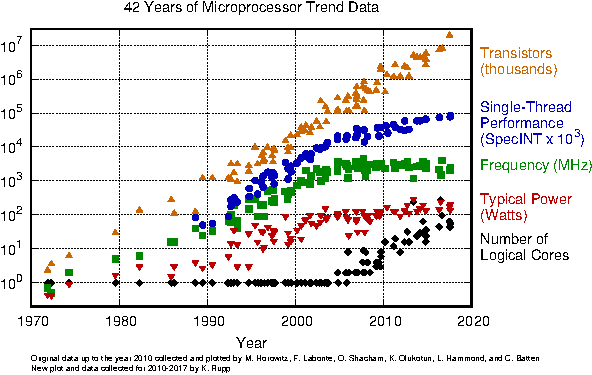
\includegraphics[width=.85\textwidth]{images/42-years-processor-trend.pdf}

		\caption{
			42 years of Multiprocessor Trend Data~\cite{url:microprocessor-trend-data}.
		}\par
		\label{fig.microprocessor-data}
	\end{figure}

% - From multicore to manycores

	However, Figure \ref{fig.microprocessor-data} shows that, in recent years,
	the energy consumption of parallel processors has become as crucial as their
	processing power, which is usually measured by the number of \flops.
	At this point, with the popularization of embedded systems as well as the aim
	to reach the \exascale (10$^{18}$ \flops), a new class of parallel processors,
	named \textit{lightweight} \manycores, emerged to provide high parallelism
	with low-power consumption.

% FROM FUNDAMENTATION
% {
	% With the enhancement of technologies and the reduction of transistors,
	% the number of cores inside a multiprocessor began to scale.
	% Until at some point, these architectures must be called \manycores.
	% However, the line between multi-cores and \manycores is very tenuous.
	% Some researchers stipulate that the difference lies when losing a core
	% does not impact the rest of the system.
	% In this way, \manycores are as multi-cores with tens, hundreds, or even
	% thousands of cores, presenting the most diverse architectural properties.
	% For example, there are \uma/\numa multiprocessors with \simd present on
	% \gpus, and \numa multiprocessors with \mimd as \mppa presented in Section \ref{sec.multiprocessor-hw}.

	% A promising class of \manycores began to emerge, aiming the energy barrier
	% that we will face in the future.
	% \textit{Lightweight Manycores} stand out for their performance compared
	% to their energy consumption.
	% However, due to its particular characteristics, several problems of
	% programmability, portability, and performance are still open.
% }

% - Manycores characteristics
	The \textit{lightweight} \manycores
		(i) integrate thousands of low-power cores in a single die organized in clusters;
		(ii) are designed to cope with \mimd workloads;
		(iii) rely on a high-bandwidth \noc for fast and reliable message-passing communication;
		(iv) present constrained memory systems; and
		(v) frequently feature a heterogeneous configuration.
	Some industry-successful examples of \textit{lightweight} \manycores are
	the \mppa~\cite{DeDinechin2013-1};
	the \epiphany~\cite{olofsson2014}; and
	the \taihulight~\cite{zheng2015}.

% Motivation
% - Difficults from Manycores
	Jointly with further performance scalability and energy efficiency, manycores brought a new
	set of challenges in software development coming from their architectural particularities.
	Precisely, these particularities introduce the following difficulties:
	\begin{itemize}
		\item \textbf{Hybrid programming model:} due to the parallel and distributed nature of
			the architecture, engineers are frequently required to adopt a message-passing
			programming model to deal with the presence of rich \nocs~\cite{kelly2013} that
			interconnects clusters and a shared-memory model inside the cluster.
		\item \textbf{Missing hardware support for cache coherency:} to reduce power consumption,
			theses processors do not feature cache coherency, which in turn forces programmers to
			handle it explicitly in software level and frequently calls out for a redesign in their
			applications~\cite{francesquini2015};
		\item \textbf{Constrained memory system:} the frequent presence of multiple physical
			address spaces and small local memories require data tiling and prefetching to be
			handled by the software~\cite{Castro2016};
		\item \textbf{Heterogeneous configuration:} the different programmable components on
			\textit{lightweight} \manycores turns the actual deployment of applications in a
			complex task~\cite{barbalace2015}.
	\end{itemize}

% - Why is development on manycores difficult?
	Part of these challenges derives from existing \oses and runtimes.
	On the one hand, the complicated portability and scalability of traditional \oses with a
	monolithic kernels, which were designed to homogeneous hardwares, is leading to the development
	of new \oses from scratch~\cite{Baumann2009, kluge2014, nightingale2009, rhoden2011}.
	On the other hand, existing runtimes only partially address some of the programmability issues
	of \textit{lightweight} \manycores, making the process of developing, porting, and maintaining
	applications a challenging task.

% Challenges and Problem Definition
% - How are OSs essential in this context?

% - Why these problems exist? (Because the existing OSes does not handle architecture particularities)
% - These particularities prevent common OSes that easy portated without a complex redesign. And existing OSes does not account some architectural points.

% Goals and Contributions
% - Redesign from scratch around all their tight architectural constraints.
% - Focus on addressing first-order programmability challenges
% - Introducing generic and flexible HAL for lightweight manycores
	% Nexte contexto, o doutorando e coorientador deste trabalho, Pedro H. Penna, mirando a maior programabilidade e portabilidade para lightweight manycores, propoe que sistemas operacionais para essa nova geração de processadores deve ser reprojetada do zero baseando-se em todas as suas restrições arquiteturais.
	% Sua proposta envolve um sistema operacional completo distribuido baseado em uma arquitetura multikernel~\cite{multikernel}.
	% Para isso, baseados em resultados de serviços experimentais desenvolvidos encimado do mppa256~\cite{rmem}, a pesquisa começou buscando resolver os primeiros desafios que surgiram.
	% Especificamente, foi introduzido uma \hal genérica e flexivel para lightweight manycores que lidam com os problemas chaves encontrados no desenvolvimento para esses processadores.
	% Em seguida, a pesquisa seguirá em desenvolver um microkernel para prover os mecanismos básicos para desenvolvimento de um OS completo sobre ele.
	% Por fim, o desenvolvimento de serviços do multikernel serão alcançados.

	We believe that \oses for the next-generation of \textit{lightweight} \manycores must be
	redesigned from scratch to cope with their tight architectural constraints.
	Based on this idea, a new fully-featured distributed \os based on a \multikernel approach~\cite{Baumann2009}
	is being proposed~\cite{penna2017-1,penna2017-2,penna2019}.
	Nanvix features a generic and flexible \hal for \textit{lightweight} \manycores that
	addresses the key issues encountered in the development for these processors.
	On top of the Nanvix \hal, we are simultaneously designing and implementing a \microkernel
	that provides bare bones system abstractions for each cluster.

	In this monograph, we intend to propose a Inter-Cluster Communication Module to the Nanvix \hal
	and port it to the \mppa manycore processor~\cite{DeDinechin2013-1}.
	Using this module, we also pretend design Inter-Cluster Communication Services to the Nanvix \microkernel.
	This work will be done in collaboration with Pedro H. Penna, who is a Ph.D. student at the
	University of Grenoble Alpes, the main developer of Nanvix and the co-advisor of this work.
	Then, we will analyze the performance of the proposed implementation using specific micro-benchmarks.

\section{Objectives}

	This will be written last.
%    Assist to research and develop \hal for \textit{lightweight} manycores.

\subsection{General Objective}

	This will be written last.
%    On the basis of the foregoing, the following general objective and the specific objectives of this project.

\subsection{Specific Objectives}
   \begin{itemize}
		\item This will be written last.
    %    \item Present and discuss hal \textit{lightweight} manycores.
    %    \item Design and develop the Inter-cluster communication module.
    %    \item Assist in the development and improvement of other modules.
    %    \item Perform a performance analysis of the proposed \hal for the \mppa.
   \end{itemize}

\section{Organization Of The Work}

	This will be written last.
\chapter{Background}
\label{ch.fundamentation}

	This chapter presents the background of multiple processor
	systems from a hardware and software perspective.
	Specifically, \autoref{sec.multiprocessors} and \autoref{sec.multicomputers}
	will address details about multiprocessors and multicomputers, respectively.
	Subsequently, \autoref{sec.mppa} will present the \mppa processor.
	Next, \autoref{sec.nanvix} will show an overview of the Nanvix OS.
	So finally, \autoref{sec.inter-cluster-communication} will cover the abstraction
	concepts in the Inter-Cluster Communication Module.

\section{Multiple Processor Systems}
\label{sec.multiple-processor-systems}

	According to Tanenbaum~\cite{tanenbaum:4ed}, there are three models of
	modern multiple processor architectures.
	A shared-memory multiprocessor, a message-passing multicomputer, and a wide
	area distributed systems.
	The sections below address the two first models presenting significant
	hardware and software concepts for the present undergraduate dissertation.

	\subsection{Multiprocessors}
	\label{sec.multiprocessors}

		\begin{figure}[t]
			\centering%
			\caption{Von Neumann Architecture Model.}%
			\label{fig:neumann}%
			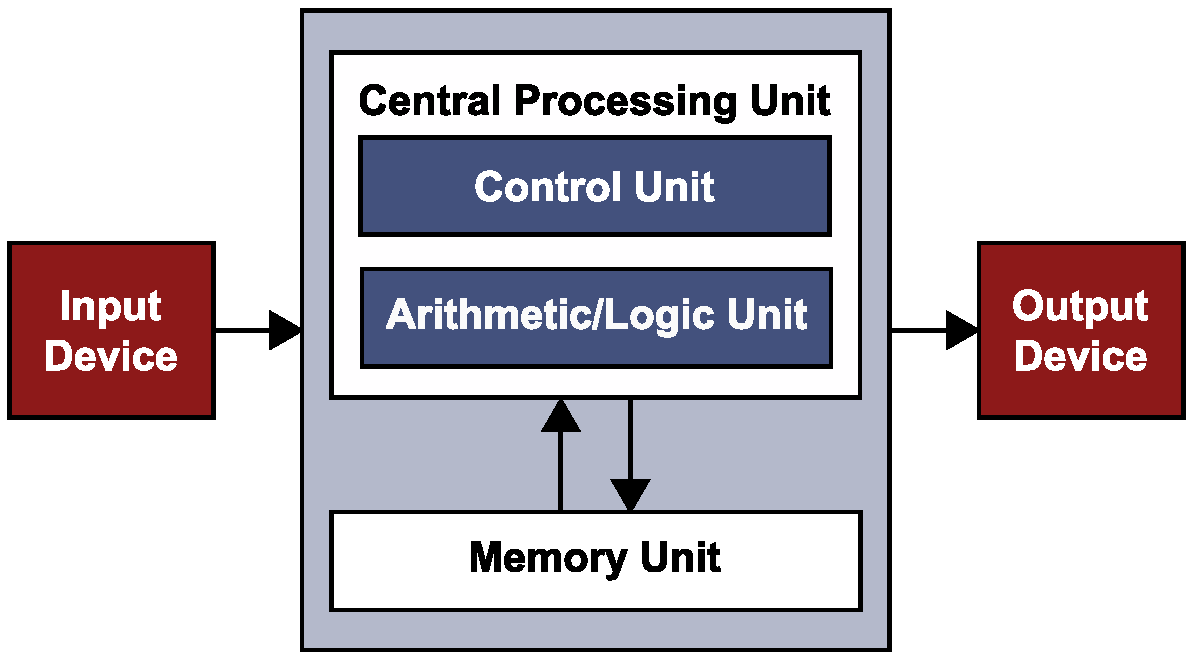
\includegraphics[width=.7\textwidth]{neumann.pdf}%
			\fonte{Adapted from \citeonline{tanenbaum:4ed}.}%
		\end{figure}

		In the early days of electronic digital computing, John Von Neumann
		proposed an architectural model for computers to be easily programmable~\cite{von-neumann:model}.
		As illustrated in \autoref{fig:neumann}, this model describes a \cpu,
		also called core, that loads instructions and data from a \mmu,
		dealing with inputs and generating outputs from/to I/O Devices.
		Modern processors still follow this model, but some components and
		behaviors are specialized or replicated to increase performance.

		In this context, a shared-memory multiprocessor is a computer system
		in which two or more \cpus share full access to a common \ram~\cite{tanenbaum:4ed}.
		Concurrency issues begin to appear where are many \cpus competing for
		shared resources.
		For instance, when many threads of a process competing to read and write a global variable.
		Moreover, some architectures integrate heterogeneous cores introducing portability
		and programmability problems too.
		So, low-level software, such as \os kernels and runtimes, needs to handle those
		issues and provide management systems to user-level.

		\subsubsection{Multiprocessor Hardware}
		\label{sec.multiprocessor-hw}

			The multiprocessors can be usually classified using memory access
			and workflow properties.
			In the first place, the access time to different memory addresses
			split multiprocessors into two groups.
			On the one hand, the group of systems that can read a memory word
			as fast as every other memory word are called \uma multiprocessors.
			On the other hand, \numa multiprocessors do not have this property.

			\begin{figure}[t]
				\centering%
				\caption{Two Bus-Based \uma Multiprocessor Examples.}%
				\label{fig:uma}%

				\subcaptionminipage[fig:uma_a]%
					{.4\linewidth}%
					{Without caching.}%
					{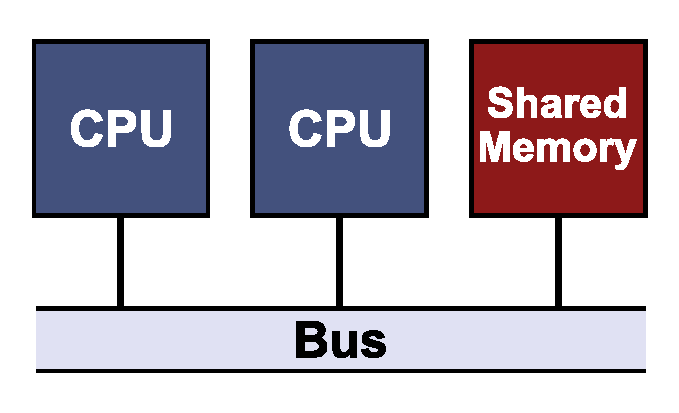
\includegraphics[width=\linewidth]{uma_a.pdf}}%
				\hspace{1.5cm}%
				\subcaptionminipage[fig:uma_b]%
					{.4\linewidth}%
					{With caching.}%
					{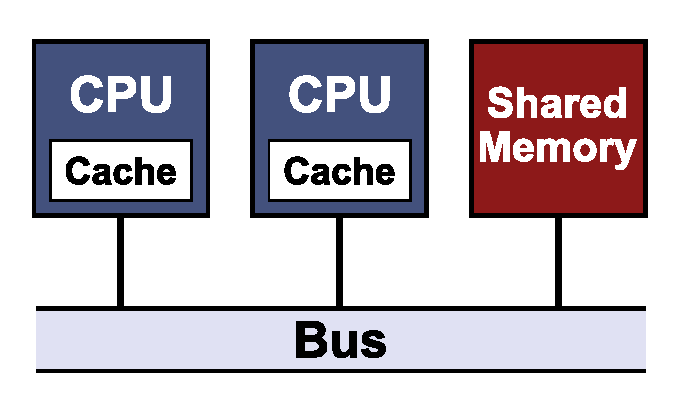
\includegraphics[width=\linewidth]{uma_b.pdf}}%

				\fonte{Adapted from \citeonline{tanenbaum:4ed}.}%
			\end{figure}

			The firsts \uma multiprocessors were bus-based architectures where
			the \cpu wait for the bus channel stays free to perform a memory
			access, as illustrated in \autoref{fig:uma}(a).
			When the number of cores scale, the bus traffic begin to be a
			bottleneck of the system.
			To solve this problem, a small but fast memory level, called cache,
			is added to each \cpu, as depicted in \autoref{fig:uma}(b).
			The cache allowed readings to be resolved locally, reducing traffic
			to the main memory.
			However, many problems of inconsistency and ordering of operations
			on memory arose with the advent of caches.
			For instance, when a write operation dirties a memory address in
			a particular cache, this change must be notified to all other caches.
			Equally important, it is necessary to ensure a specific order in
			the concurrent operations on a given address through different caches.
			The protocols that guarantee these properties are called cache-coherence protocols.

			\begin{figure}[t]
				\centering%
				\caption{\numa Multiprocessor Example.}%
				\label{fig:numa}%
				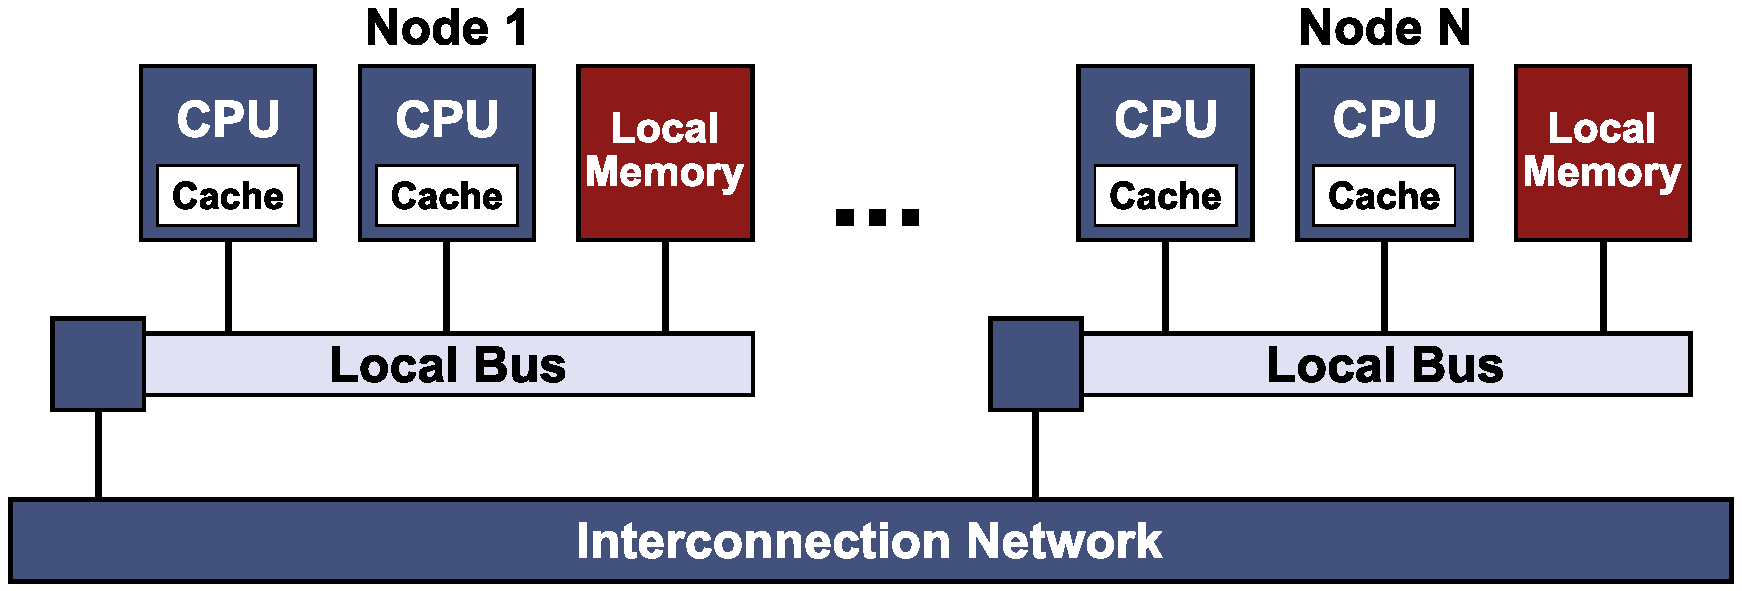
\includegraphics[width=.7\textwidth]{numa.pdf}%
				\fonte{Adapted from \citeonline{tanenbaum:4ed}.}%
			\end{figure}

			Nevertheless, the number of cores in \uma multiprocessors are limited
			to a few dozens of \cpus.
			Thus, to allow hundreds of cores to communicate, \autoref{fig:numa} illustrated
			as that \numa machines provide a single address space visible to all \cpus
			through an interconnection network.
			Therefore, distributing a virtual memory space among local physics memories,
			the access is guaranteed via load and store instructions.
			Although the time to access to remote memory is slower than to local ones,
			this granted that all \uma programs will be able to run on \numa machines
			but with worse performance.

			\begin{figure}[t]
				\centering%
				\caption{Flynn's taxonomy.}%
				\label{fig:flynn}%
				
				\subcaptionminipage[fig:flynn-sisd]%
					{.4\linewidth}%
					{Single Instruction Single Data.}%
					{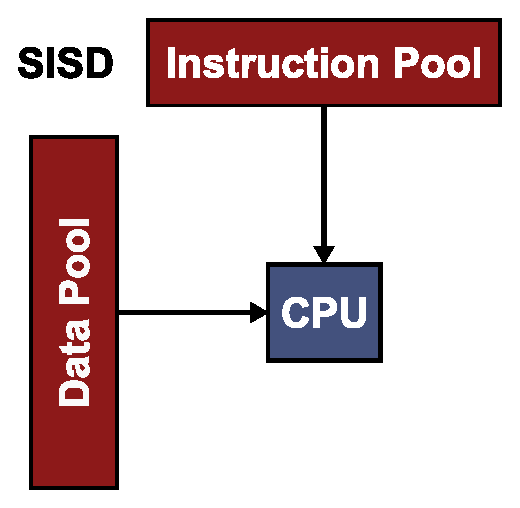
\includegraphics[width=.8\linewidth]{sisd.pdf}}%
				\hspace{1cm}%
				\subcaptionminipage[fig:flynn-simd]%
					{.4\linewidth}%
					{Single Instruction Multiple Data.}%
					{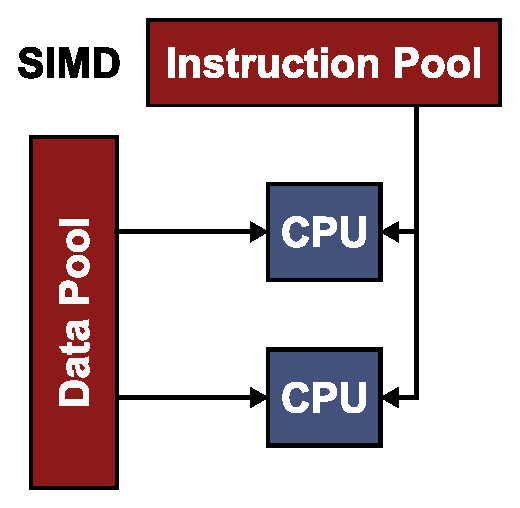
\includegraphics[width=.8\linewidth]{simd.pdf}}%

				\subcaptionminipage[fig:flynn-misd]%
					{.4\linewidth}%
					{Multiple Instruction Single Data.}%
					{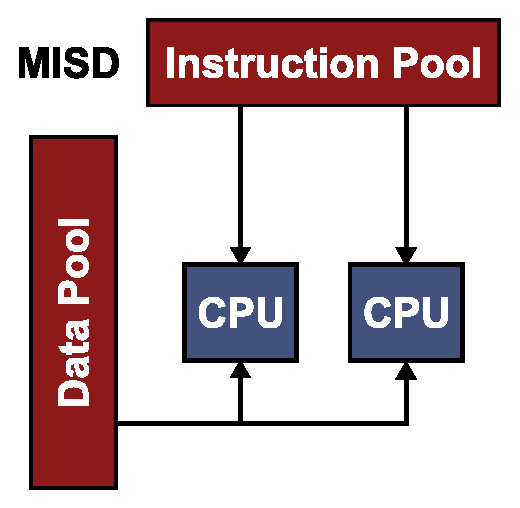
\includegraphics[width=.8\linewidth]{misd.pdf}}%
				\hspace{1cm}%
				\subcaptionminipage[fig:flynn-mimd]%
					{.4\linewidth}%
					{Multiple Instruction Multiple Data.}%
					{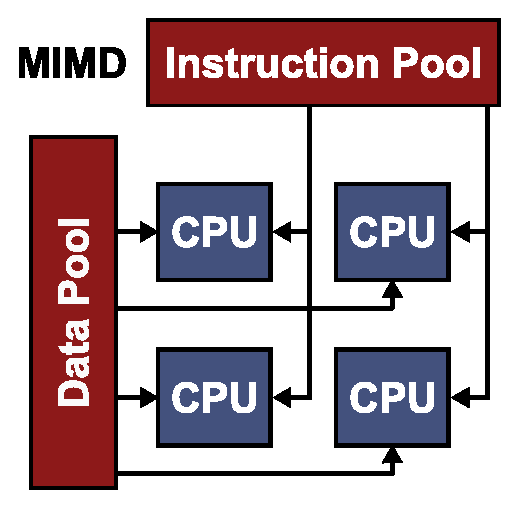
\includegraphics[width=.8\linewidth]{mimd.pdf}}%

				\fonte{Adapted from \citeonline{url:flynn}.}%
			\end{figure}

			In the second place, the workflow classification proposed by Michael J. Flynn~\cite{flynn:1972},
			split multiprocessors architecture based on the number of concurrent
			instruction and data streams available, as depicted in \autoref{fig:flynn}.
			First, the most straightforward class, \sisd describes a sequential
			machine which exploits no parallelism in either the instruction or
			data streams, like older uniprocessor machines.
			Second, \simd uses multiple functional units to replicate and operate
			a single instruction over multiples different data streams, like \gpu.
			Third, the most uncommon class, \misd describe multiprocessors that
			apply multiple instructions streams over one data stream.
			Systems that need fault tolerance uses theses multiprocessors, like
			modern flight control systems.
			Finally, a \mimd architecture has multiple processors simultaneously
			executing different instruction on different data, like \xeonphi.

			Currently, two categories of multiprocessors attract attention, the \cmp and \mpsoc.
			\cmps are multicore commercials, which follow a symmetric architecture,
			integrating two or more identical cores into a single die.
			They can have private or shared cache levels, and always share access
			to the RAM.
			Alternatively, \mpsocs are designed with an asymmetric architecture,
			have in addition to the main cores, specialized \cpus in particular
			functions, \eg audio and video encoders, encryption, becoming truly
			complete computer systems on a single chip.
			All these cores are linked to each other by an on-chip network-based
			communications subsystem, called \noc.
			The \noc improve scalability and power consumption compared to other
			communication subsystem designs.

		\subsubsection{Multiprocessor \oss}
		\label{sec.multiprocessor-os}

			\oss are a fundamental part of any computer system.
			They act as an intermediary between users and hardware, with the
			purpose to provide an environment in which users can run programs
			in a conveniently and efficiently manner~\cite{Silberschatz:9ed}.
			Many \os approaches exist in multiprocessor systems.
			In particular, three of them express accurately the difficulties
			of developing \oss targeting the concurrency issues existing in
			such systems.
			Those models are called Replicated, Master-Slave, and Symmetric \os.

			\begin{figure}[t]
				\centering%
				\caption{Replicated \os Model.}%
				\label{fig:replicated-os}%
				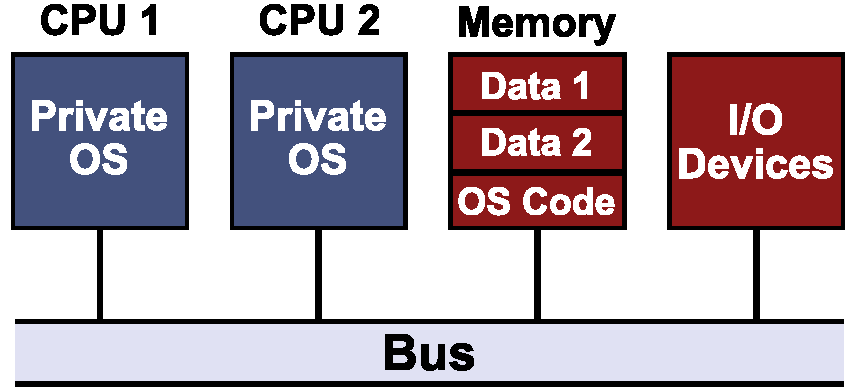
\includegraphics[width=.55\textwidth]{replicated-os.pdf}%
				\fonte{Adapted from \citeonline{tanenbaum:4ed}.}%
			\end{figure}

			The Replicated Model is the simplest way to develop an \os for a
			parallel architecture.
			It only needs to replicate all the internal \os structures for each core.
			\autoref{fig:replicated-os} shows how this model allocates fixed memory spaces
			between the cores, giving each of them its private \os.
			The system calls are performed by the calling \cpu, avoiding concurrency issues.
			Also, a producer-consumer model is sufficient for two different \cpus to communicate.

			However, this model has imperceptible aspects~\cite{tanenbaum:4ed}.
			First, since each \cpu has its own process and page tables, it is impossible
			to optimize the use of resources.
			For instance, if many of processes are waiting for use an overloaded \cpu,
			it is impossible to migrate them to an available \cpu.
			Second, operations with I/O devices can introduce inconsistency problems
			such as the same disk block operated by different \cpus.
			Finally, replication of the internal \os structures makes this model
			impractical for systems with memory constraints.

			\begin{figure}[t]
				\centering%
				\caption{Master-Slave \os Model.}%
				\label{fig:master-slave-os}%
				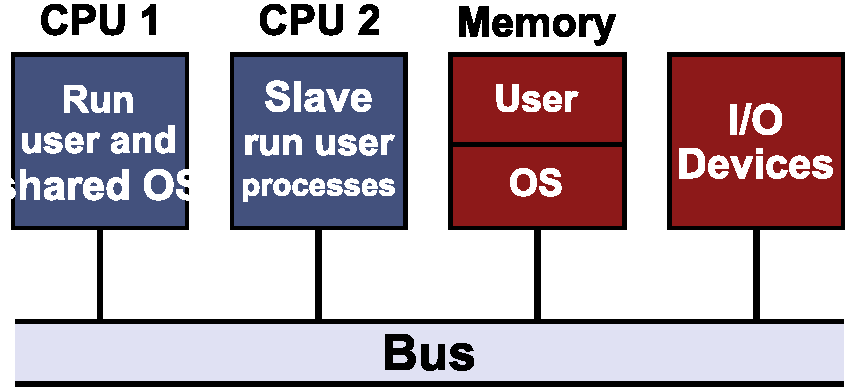
\includegraphics[width=.55\textwidth]{master-slave-os.pdf}%
				\fonte{Adapted from \citeonline{tanenbaum:4ed}.}%
			\end{figure}

			The Master-Slave model began to attract attention with the return of
			processors with no cache coherence.
			As \autoref{fig:master-slave-os} shows, there is only one copy of
			the internal \os structures, and they all belong to a single \cpu, called master.
			In this way, all system calls performed by a worker \cpu, called slave,
			are redirected to the master.
			With these changes, this model solves the problems of the previous model
			by using only one copy of the data structures.
			For illustration, processes and memory pages can be scheduled and
			distributed dynamically to any \cpus.
			However, when adopting a centralized approach, the master can become
			the bottleneck of the system if it can not handle the number of the
			incoming requisition.

			\begin{figure}[t]
				\centering%
				\caption{Symmetric \os Model.}%
				\label{fig:smp-os}%
				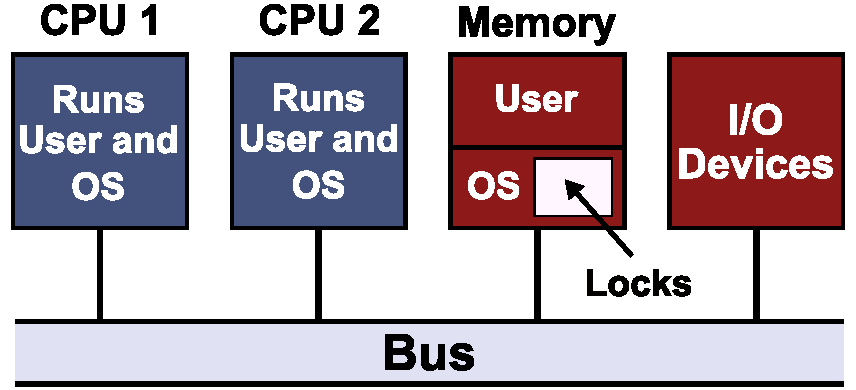
\includegraphics[width=.55\textwidth]{symmetric-os.pdf}%
				\fonte{Adapted from \citeonline{tanenbaum:4ed}.}%
			\end{figure}

			Finally, the Symmetric model, called \smp, eliminates the centralization
			problem of the foregoing model, as illustrated in \autoref{fig:smp-os}.
			So, there is still only one copy of the \os structures but shared in memory.
			When a \cpu makes a system call, it loads the structures and operates on them.
			Consequently, processes and memory pages also continue to be dynamically balanced.
			The difficulties introduced by this model lie in concurrency for \os structures.
			Depending on how the critical regions are managed, the performance of the system
			may be equivalent to the Master-Slave model. So the hardest part is breaking the
			\os into critical regions that will run on different \cpus, where one core does
			not affect the execution of another or fall into a deadlock~\cite{tanenbaum:4ed}.
			Besides, if the hardware does not support cache coherence, the process of
			invalidating the cache may also introduce serious performance problems in \oss of this type.

			As it can be noted, the software is always lagging behind the constant hardware advances.
			Many solutions may work very well in specific contexts but should be chosen with care.
			In some cases, in order to extract the maximum performance from a system, it will be
			necessary to redesign the whole process from scratch.

	\subsection{Multicomputers}
	\label{sec.multicomputers}

		Increasing the number of cores and still providing a shared memory in a
		single die is very expensive and challenging.
		However, it is more simple and cheap to interconnect more straightforward
		computers in a high-speed network. The result is a clustered archietcture.
		Despite the problem of developing networks and high-speed interfaces
		for communication of the nodes, it is analogous to the problem of
		providing a shared memory in multiprocessors.
		Nevertheless, the expected communication times will be in the
		microseconds, as opposed to nanoseconds of the multiprocessors,
		making things simpler~\cite{tanenbaum:4ed}.

			\subsubsection{Multicomputer Hardware}
			\label{sec.multicomputers-hw}

				A multicomputer node can be considered as an elementary computer, with one or
				more multiprocessors, local \ram and I/O devices.
				In many cases, there is no need for monitors or keyboards, only the
				network interface.
				In this way, it is possible to integrate hundreds or even thousands
				of nodes providing the vision of a single computer.

				\begin{figure}[t]
					\centering%
					\caption{Network Topologies Examples.}%
					\label{fig:net-topologies}%

					\subcaptionminipage[fig:net-start]%
						{.25\linewidth}%
						{Star.}%
						{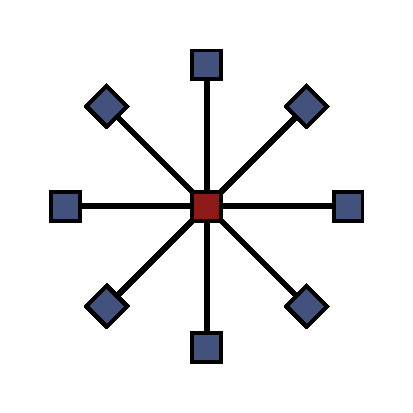
\includegraphics[width=\linewidth]{net-star.pdf}}%
					\hspace{1cm}%
					\subcaptionminipage[fig:net-ring]%
						{.25\linewidth}%
						{Ring.}%
						{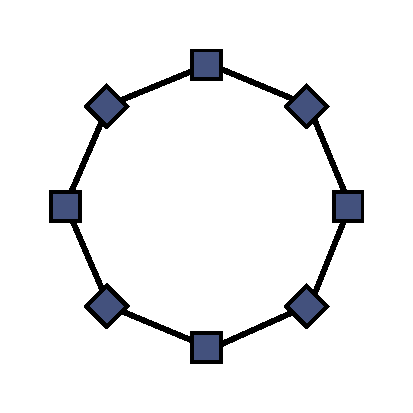
\includegraphics[width=\linewidth]{net-ring.pdf}}%
					\hspace{1cm}%
					\subcaptionminipage[fig:net-grid]%
						{.25\linewidth}%
						{Grid.}%
						{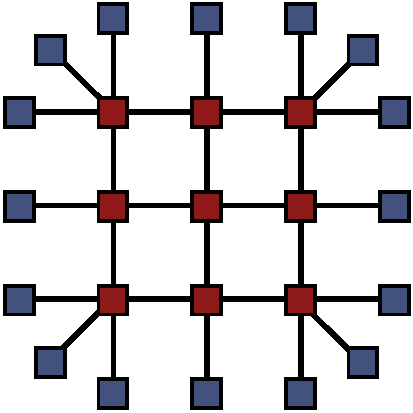
\includegraphics[width=\linewidth]{net-grid.pdf}}%

					\subcaptionminipage[fig:net-torus]%
						{.25\linewidth}%
						{Torus.}%
						{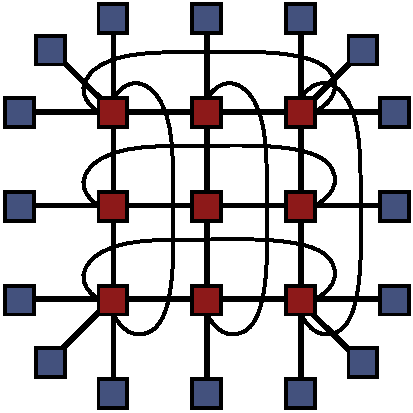
\includegraphics[width=\linewidth]{net-torus.pdf}}%
					\hspace{1cm}%
					\subcaptionminipage[fig:net.grid-3d]%
						{.25\linewidth}%
						{Grid 3D.}%
						{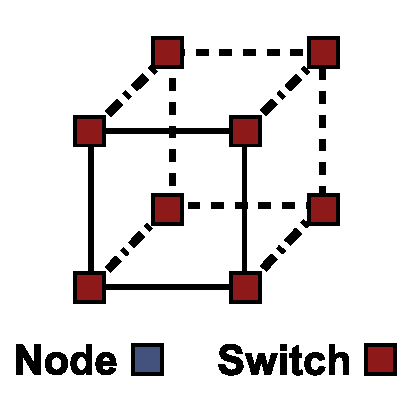
\includegraphics[width=\linewidth]{net-3d.pdf}}%

					\fonte{Adapted from \citeonline{tanenbaum:4ed}.}%
				\end{figure}

				A switch set is organized into different topologies to interconnect
				the nodes of a multicomputer.
				As illustrated in \autoref{fig:net-topologies}, there are a
				variety of topologies with their own characteristics.
				For instance, commercial multicomputer usually uses bi-dimensional
				topologies such as \textit{grid} or \textit{mesh} because they present
				regular behavior and can scale easily.
				When the goal is to provide higher fault tolerance, in addition to the
				smaller path between two points, the \textit{torus} variant implement
				connections between the extreme points of the \textit{grid}.
				Even multi-dimensional topologies can be used, all depending on the
				characteristics expected from the network.

				There are two types of switching schemes in the multicomputer network.
				The \textit{store-and-forward packet} switching scheme breaks the message
				into fixed-size packets.
				The packets are copied and moved between the switches following a
				routing algorithm until they reach the destination.
				Although flexible and efficient, this scenario can generate a variable
				latency in packet delivery.
				The other scheme, called \textit{circuit switching}, performs a resource
				allocation protocol through all path from source to the destination.
				This protocol ensures a steady communication stream, although the
				slow start and possible sub-utilization of the resources.

			\subsubsection{Low-Level Communication Software}
			\label{sec.multicomputers-low-sw}

				\begin{figure}[t]
					\centering%
					\caption{Simple Multicomputer Example.}%
					\label{fig:multicomputer}%
					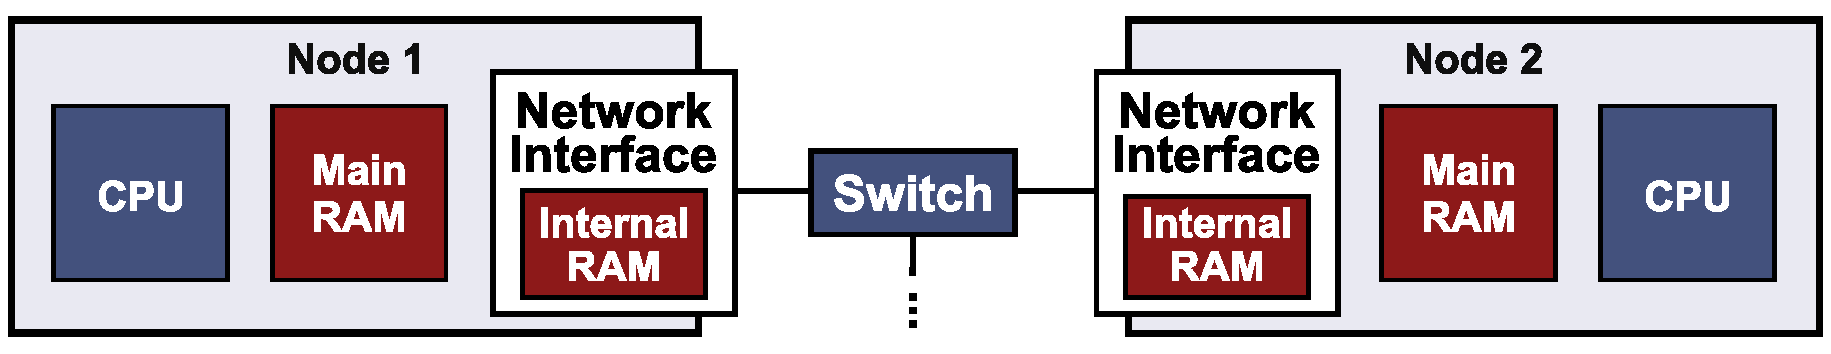
\includegraphics[width=.8\textwidth]{multicomputer.pdf}%
					\fonte{Adapted from \citeonline{tanenbaum:4ed}.}%
				\end{figure}

				Multicomputer nodes are interconnected to each other through network interfaces.
				Because these boards are built and connected to \cpus and \ram,
				they have substantial impacts on system performance and \os design.
				Virtually, interfaces have enough \ram space to receive/send packets.
				If this address space is actually in main memory, we fall into the same
				problem of multiprocessors in the struggle for the use of the bus channel.
				Thus, in general, network cards have a dedicated memory so as not to
				generate bottlenecks in access to main memory, as illustrated in \autoref{fig:multicomputer}.

				However, excessive packet copying can degrade the performance of the system.
				In an ideal scenario, four end-to-end copies would be needed:
				(i) from the \ram of the sender to the interface memory;
				(ii) from the interface to the network;
				(iii) from the network to the memory of the target interface, and, finally,
				(iv) to the \ram of the recipient.
				However, the number of copies may increase further, depending on how the \os
				implements communication services on available hardware.
				For instance, mapping the interface into the kernel address space
				rather than the user-space, an extra copy to an internal kernel
				buffer is required.
				Thus, for performance reasons, modern systems already map the interfaces
				to user-space address.
				Nonetheless, they introduce problems of concurrency between the various
				users by the communication resources.

				Processors may also have one or more \cpus specialized in
				communication procedures, called \dma.
				\dmas can make copies between system memories, send/receive packets
				without the main \cpus intervention. This reduces considerably wasted cycles due to 
				network interfaces communication and/or main memory access bottlenecks.
				However, such intermediate copies lead to overhead on system structures,
				such as cache, \tlb, or page management.
				Furthermore, this introduces concurrency issues in the interaction between
				\cpus and existing \dma channels.

			\subsubsection{User-Level Communication Software}
			\label{sec.multicomputers-user-sw}

				The low-level mechanisms discussed above allow \cpus on different
				computers to communicate through the messages exchange by
				send/receive primitives.
				The basic configuration needed for send primitive is knowing the
				recipient identifier and the message.
				Moreover, the receive primitive needs to identify which of
				the network interfaces it should configure and where to write the
				incoming data.

				\begin{figure}[t]
					\centering%
					\caption{Calls Types.}%
					\label{fig:calls-types}%

					\subcaptionminipage[fig:call-sync]%
						{.9\linewidth}%
						{Synchronous Call on Sender Node.}%
						{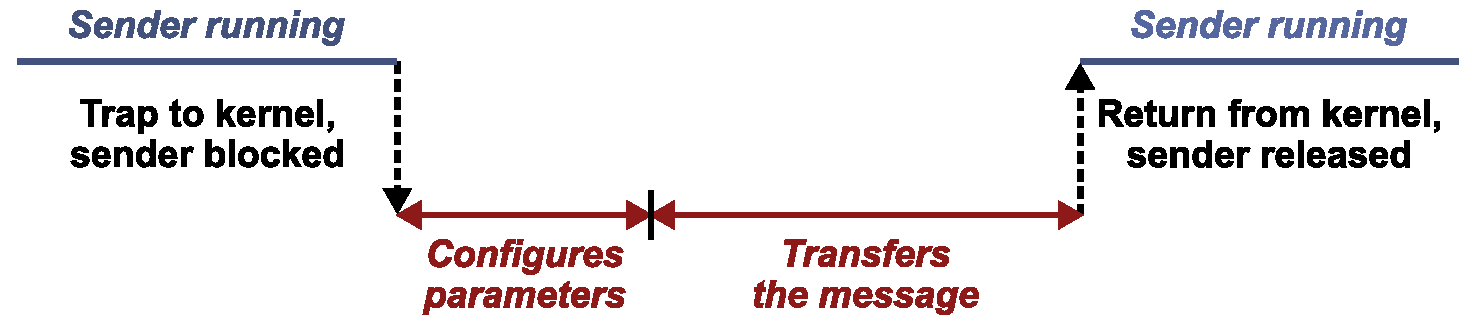
\includegraphics[width=\linewidth]{call-sync.pdf}}%

					\hfill

					\subcaptionminipage[fig:call-async]%
						{.9\linewidth}%
						{Asynchronous Call on Sender Node.}%
						{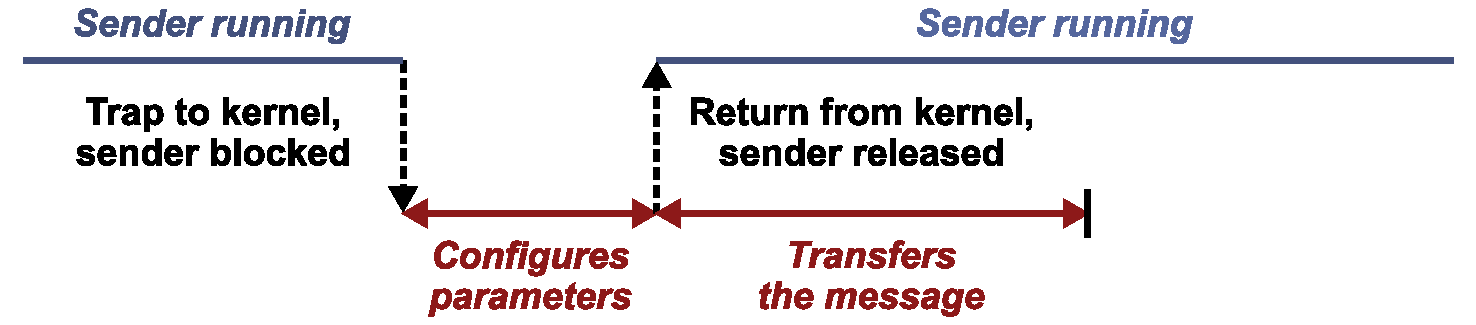
\includegraphics[width=\linewidth]{call-async.pdf}}%

					\fonte{Adapted from \citeonline{tanenbaum:4ed}.}%
				\end{figure}

				\autoref{fig:calls-types} illustrates the two approaches to implement
				these primitives, either through blocking or non-blocking calls.
				Blocking calls, called \textit{synchronous calls}, block the requesting \cpu
				until complete the procedure.
				Non-blocking calls, called \textit{asynchronous calls}, return control to the
				\cpu while the procedure is still in progress.
				Although asynchronous calls provide better performance than
				synchronous ones, they introduce some disadvantages where the sender/receiver
				cannot use the message buffer before the operation is complete.
				According to Tanenbaum~\cite{tanenbaum:4ed}, there are four ways to implement
				a send primitive:
				\begin{itemize}
					\item \textit{Blocking sending:} \cpu hibernates or schedules another
						process, while the message is transmitted;
					\item \textit{Non-blocking sending with copying:} realizes an extra copy of
						the message to a kernel buffer, degrading performance;
					\item \textit{Non-blocking sending with interrupt:} notifies the \cpu
						when the send finishes, where the buffer must remain untouchable,
						difficulting the programmability;
					\item \textit{\cow:} management of buffers to make an extra copy only
						when needed, but can copy unnecessarily.
				\end{itemize}

				Analogously, there are other four forms to implement a receive primitive:
				\begin{itemize}
					\item \textit{Blocking receive:} \cpu hibernates or schedules another
						process until a message is received;
					\item \textit{Non-Blocking receive with messages pool:} \cpu creates
						a buffer to store incoming messages, then consumes from it when
						there is some message available, requiring synchronization;
					\item \textit{Non-Blocking receive with Pop-up Threads:} creates a specific
						thread upon receiving a message to perform the necessary operations,
						but consumes resource for creating and destroying the thread;
					\item \textit{Non-Blocking receive with interrupt handlers:} the receiver
						is interrupted to execute a handler when receiving a message, resulting
						in a better performance than creating a thread but difficults
						the programmability.
				\end{itemize}

				Some of the implementation approaches may be hardware dependent.
				However, choosing the ideal approach is still the responsibility of the \os designer.
				Even so, the distributed nature of multicomputers forces developers to
				use a messaging strategy regardless of what the hardware has to offer.

\section{The MPPA-256 Lightweight Manycore Processor}
\label{sec.mppa}

	\begin{figure}[t]
		\centering%
		\caption{Architectural overview of the \mppa processor.}%
		\label{fig:mppa-arch}%
		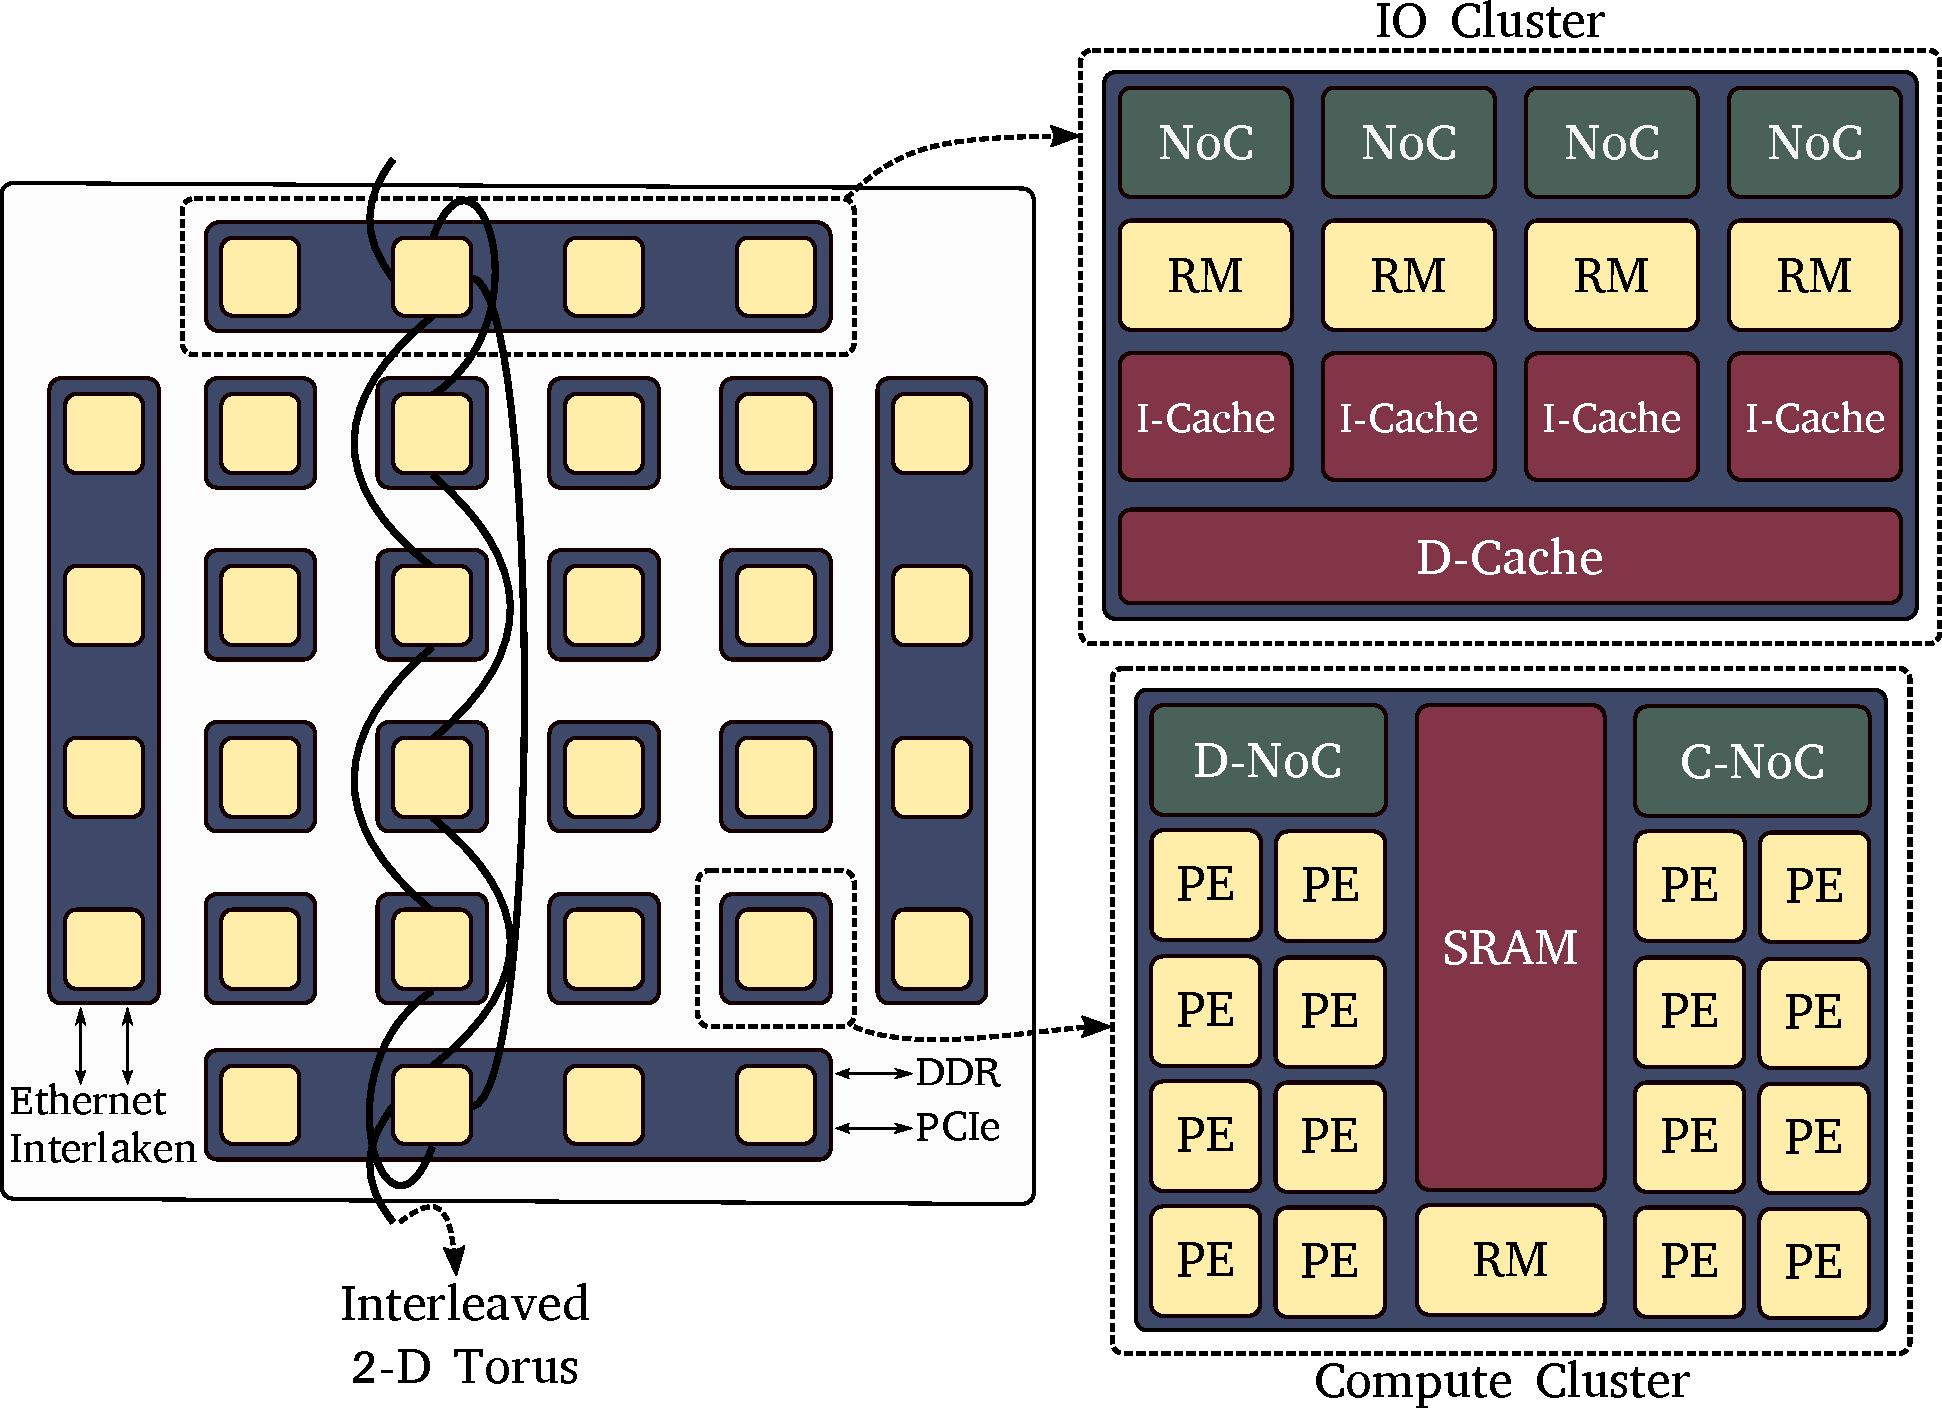
\includegraphics[width=.7\textwidth]{arch-mppa.pdf}%
		\fonte{\citeonline{Penna2018}.}%
	\end{figure}

	The \mppa is a high-performance, lightweight multicore processor
	developed by the French company Kalray.
	Developed to handle \mimd workloads, \mppa mixes features of
	multiprocessors and multicomputers on a single chip.
	Precisely, the multiprocessor model is used inside a cluster
	to coordinate the cores and the local resource balancing, and
	follows a multicomputer model in inter-cluster communication.

	As illustrated by \autoref{fig:mppa-arch}, the used version of
	the architecture, called Bostan, has 256 general-purpose cores and
	32 firmware cores, called \pes and \rms, respectively.
	The processor use 28~mm CMOS technology and all cores run at 500~MHz.
	Besides, all cores have caches and \mmus with software-managed \tlbs.
	Finally, the 288 cores are grouped into 16 \cclusters, dedicated to
	the payload, and 4 \ioclusters, responsible for communicating with peripherals.

	Each \ccluster features 16 \pes, an \rm, an \noc interface and 2~MB of \sram.
	The hardware does not support cache coherence to improve energy consumption.
	On the other hand, \ioclusters have only 4 \rms with cache coherence support,
	4 \noc interfaces, and 4~MB of local \sram added to 4~GB of \dram.
	The address space on each cluster is private, forcing exchange messages
	by one of two different interleaved 2-D Torus \nocs.
	On the one hand, the \cnoc is exclusive to 64-bit control messages,
	usually used for synchronization.
	On the other hand, intense exchange data occurs through the \dnoc.
	Additionally, all clusters have available \dmas associated with each
	\noc interfaces to handle communication issues.

	As discussed in \autoref{sec.multicomputers-user-sw}, the \noc interfaces
	expose communication resource to perform send and receive primitives
	like network interfaces.
	Accurately, they summarize the following resources:

	\begin{itemize}
		\item 128 slots for receiving commands;
		\item 256 slots for receiving data;
		\item 4 channels for sending commands;
		\item 8 channels for sending data, and;
		\item 8 $\mu$threads for sending asynchronous data (each of which must
			to be associated with a transfer channel).
	\end{itemize}

	The configuration of these features is accomplished by a mix between
	writing on \dma registers and performing syscalls to a hypervisor
	that virtualizes the \mppa hardware.

\section{Nanvix: An Operating System for Lightweight Manycores}
\label{sec.nanvix}

	Current research efforts on Nanvix \os focus on the programmability and portability
	challenges that have arisen with \textit{lightweight \manycores}~\cite{christgau2017, gamell2012, serres2011}.
	We believe that significant barriers will still arise in this scenario, and the
	solution is to rethink \os design from scratch~\cite{penna:compas19, penna2019}. 
	In this context, the Nanvix \os aims improving programmability and
	software portability in lightweight manycores by means of a fully-featured
	\posix-compliant \os~\cite{penna:compas19}.
	It follows a multi-kernel design where OS services are scattered across cores and
	interacting with user processes through a Client-Server approach.
	
	Nanvix \os can be divided into three distinct kernels, \multikernel,
	\microkernel, and \hal.
	The \multikernel is made up of high-level OS services, \eg shared memory
	regions and name resolution.
	It exports both the client and server interfaces, both developed above
	the \microkernel services.
	On top of the \hal, The \microkernel follows the Master-Slave \os model
	to avoid the problem of the lack of coherence of many manycores.
	It shall run in each cluster and provide bare bones system abstractions,
	such as thread management, thread synchronization,
	virtual memory support and communication services.
	And finally, the next section will introduce \hal.

	\subsection{Hardware Abstract Layer (HAL)}
	\label{sec.hal}

		Nanvix \os proposes a generic and flexible \hal around the
		intrinsic architectural characteristics of the \textit{lightweight \manycores}.
		In this undergraduate dissertation, we  focus on the development of \hal
		to \mppa~\cite{DeDinechin2013-1}.
		However, other efforts have also been done for other platforms such
		as~\optimsoc~\cite{Wallentowitz2013}.

		Unlike other approaches that aim to design a fully-featured \os~\cite{Baumann2009,kluge2014,nightingale2009,rhoden2011},
		the \hal belongs to one level below.
		It is the first layer on top of the hardware and should provide a standard
		view of these emerging processors for a client applications, \eg \os.
		As illustrated in \autoref{fig:hal-struct}, this \hal is structured in
		two major logic layers: \textit{Cluster Abstraction Layer} and \textit{Processor Abstraction Layer}.

		\begin{figure}[t]
			\centering%
			\caption{Structural overview of the proposed \hal.}%
			\label{fig:hal-struct}%
			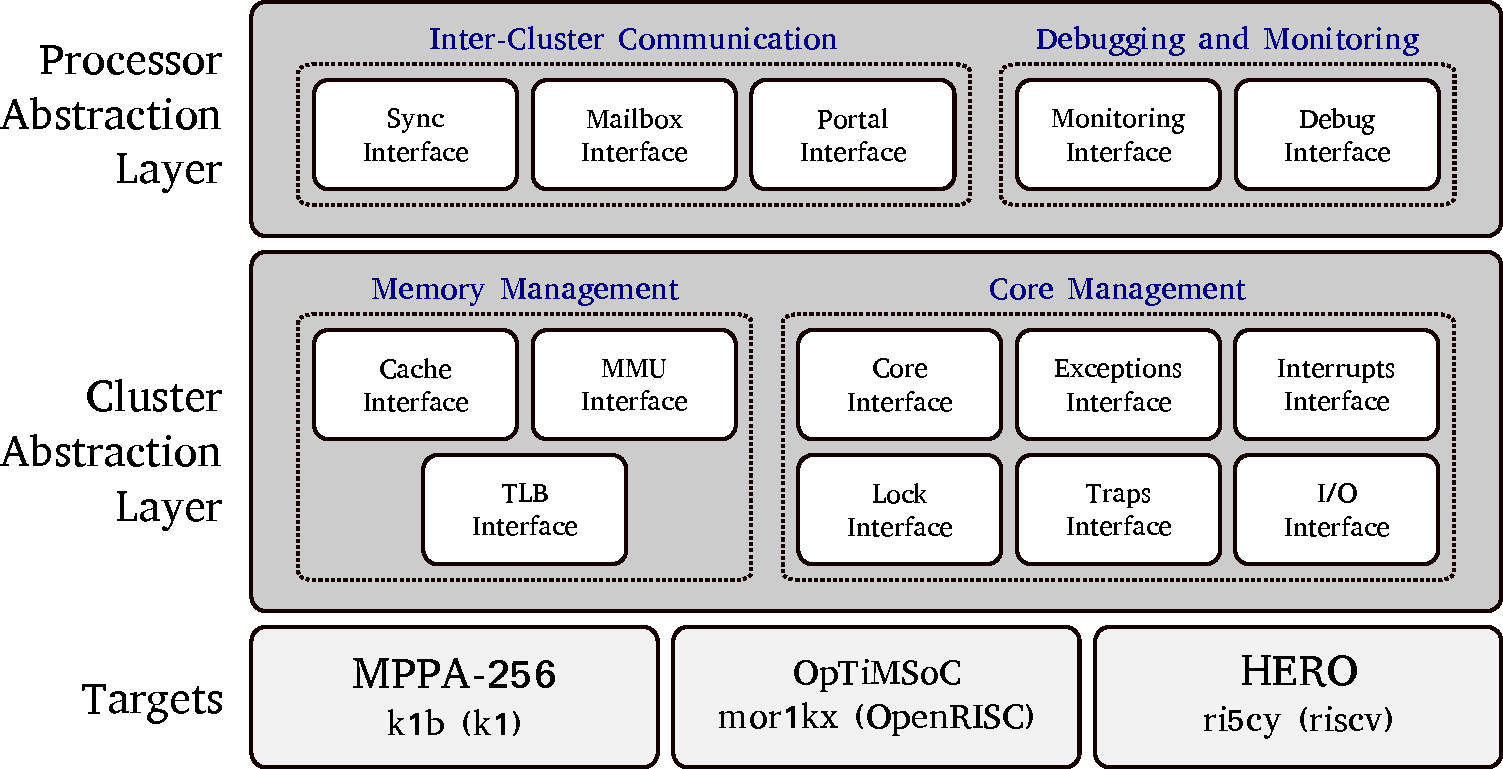
\includegraphics[width=.8\textwidth]{hal-struct.pdf}%
			\fonte{\citeonline{penna:compas19}.}%
		\end{figure}

		The \textit{Cluster Abstraction Layer} encapsulates the management of a single cluster.
		It provides two modules, \textit{Core Management}, and \textit{Memory Management}.
		The \textit{Core Management Module} aims to provide to a client application a complete
		thread synchronization and management system, rich support of handling
		interrupts/exceptions, and an adequate system call interface.
		The \textit{Memory Management Module} provides a uniform view of the \tlbs
		and paging systems with maintenance routines for them and the cache.
		Therefore, some design decisions are made to create interfaces that are not
		dependent on the underlying hardware.
		For example, a context switch mechanism was not provided in the
		Core Management module because this would force the client \os
		to write code in assembly, hurting the conceptual idea of the \hal.

		The \textit{Processor Abstraction Layer}, in particular, embraces
		architectural features related to multiple clusters.
		The \textit{Inter-Cluster Communication Module}, the focus of
		this undergraduate dissertation, exports three main abstractions to allow the
		cluster to exchange data between them, based on ideas proposed along with the
		\nodeos distributed runtime system~\cite{DeDinechin2013-1}.
		Lastly, the \textit{Monitoring and Debugging Module}, as the
		name shows, exports routines to aid debugging and extraction
		of diagnostics about hardware metrics, such as the number of
		page-fault or detour taken.

		\subsubsection{Inter-Cluster Communication Module}
		\label{sec.inter-cluster-communication}

			The following sections conceptually present the three abstractions
			exported by \hal and which will be implemented on the \mppa.
			They are the \sync, \mailbox, and \portal abstraction.
			The purpose of developing more specific abstractions than
			send and receive primitives, described in \autoref{sec.multicomputers-user-sw},
			is to provide more precise and easy-to-use mechanisms for
			\os and client applications.
			On top of them, it is possible to create all kinds of essential
			services such as message passing and synchronization,
			to more elaborate services such as shared memory regions~\cite{penna:rmen}.

			A related point to consider is that mechanisms described below refer
			to interactions between distinct clusters only.
			As described in \autoref{sec.multicomputers-user-sw}, these system
			abstractions can use the communication primitives, \ie send and receive
			primitives, to export more elaborate services.
			The behavior expected can be simulated both through synchronous calls
			and asynchronous calls, depending only on hardware support.
			In the same way, it is worth be noted that the small messaging exchange
			is decoupled from abstraction to intense data transfer.
			The motivation for this, as other details, is to exhibit better control
			over the \qos to the higher layers.
			For instance, the use of distinct \nocs for each service.

			\subsubsubsection*{Sync Abstraction}
			\label{sec.sync-abs}

				\begin{figure}[t]
					\centering%
					\caption{Synchronization Abstraction Concept.}%
					\label{fig:conpt_sync}%

					\subcaptionminipage[fig:conpt_sync-create]%
						{.7\linewidth}%
						{N Slaves notify the Master.}%
						{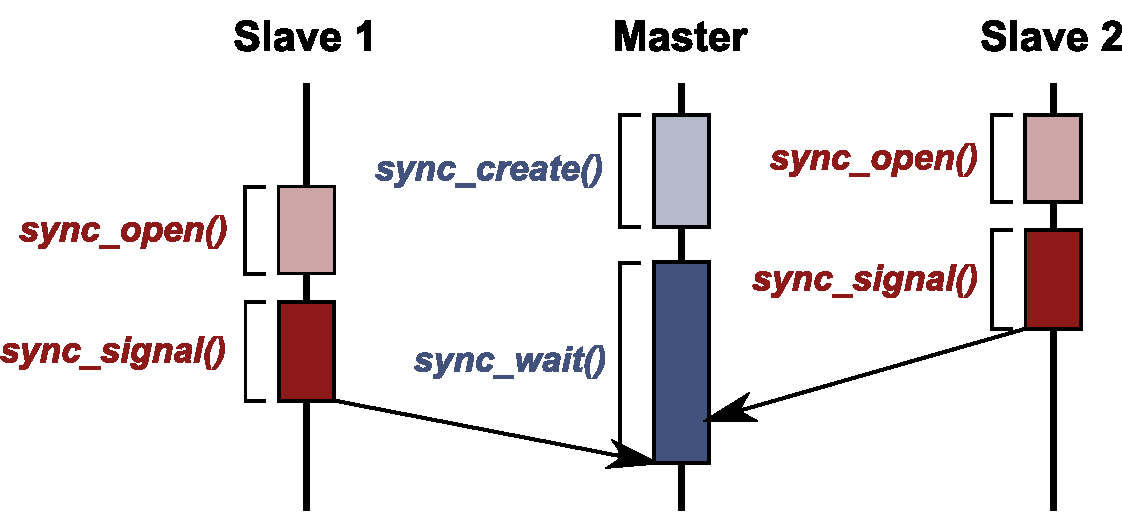
\includegraphics[width=\linewidth]{sync-create.pdf}}%

					\hfill

					\subcaptionminipage[fig:conpt_sync-open]%
						{.7\linewidth}%
						{The Master notify N Slaves.}%
						{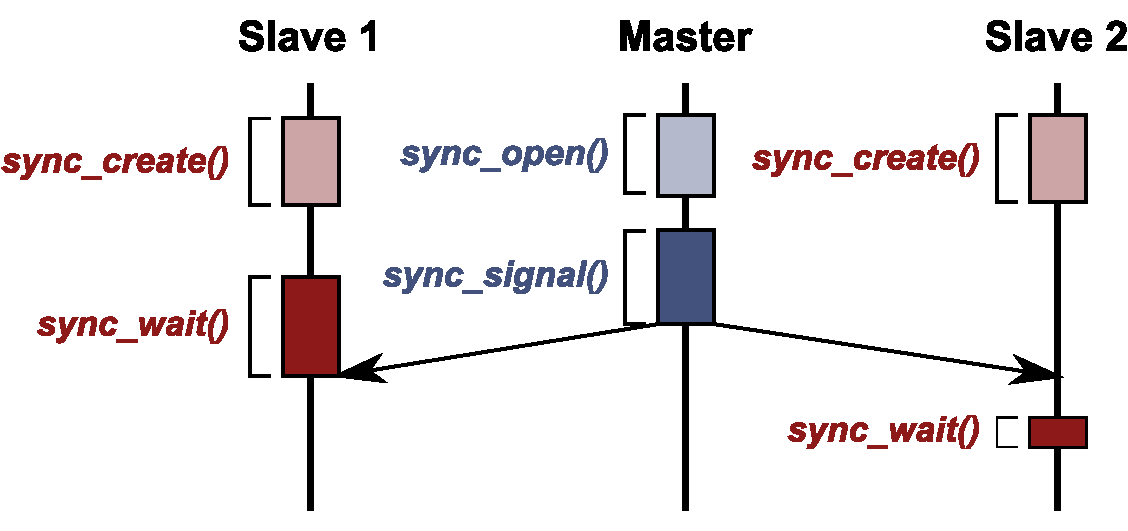
\includegraphics[width=\linewidth]{sync-open.pdf}}%

					\fonte{Developed by the Author.}%
				\end{figure}

				The \textit{Synchronization Abstraction}, called \sync, proves bare bones
				for cluster synchronization.
				From this, it is possible to create distributed barriers.
				For instance, a set of clusters can wait for a notification coming
				from a specific cluster.
				The behavior is analogous to the \posix signal abstraction, but the \sync
				provides only the case of notification.
				Specifically, as can be seen in \autoref{fig:conpt_sync}, the
				cardinality of the operation is N:1, where N clusters wait for 1 Cluster
				to send a notification.

			\subsubsubsection*{Mailbox Abstraction}
			\label{sec.mailbox-abs}

				\begin{figure}[t]
					\centering%
					\caption{Mailbox Abstraction Concept.}%
					\label{fig:conpt_mailbox}%

					\subcaptionminipage[fig:conpt_mailbox-logical]%
						{.5\linewidth}%
						{Conceptual Overview.}%
						{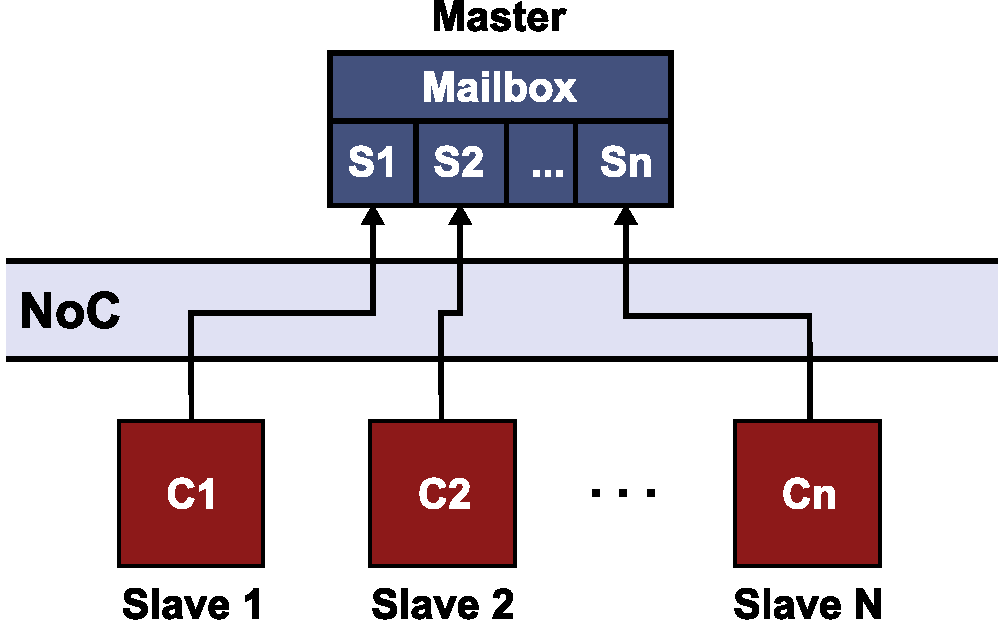
\includegraphics[width=\linewidth]{mailbox-logical.pdf}}%

					\hfill

					\subcaptionminipage[fig:conpt_mailbox-flow]%
						{.6\linewidth}%
						{Flow of execution: Slave sends a message, Master reads and notifies the sender.}%
						{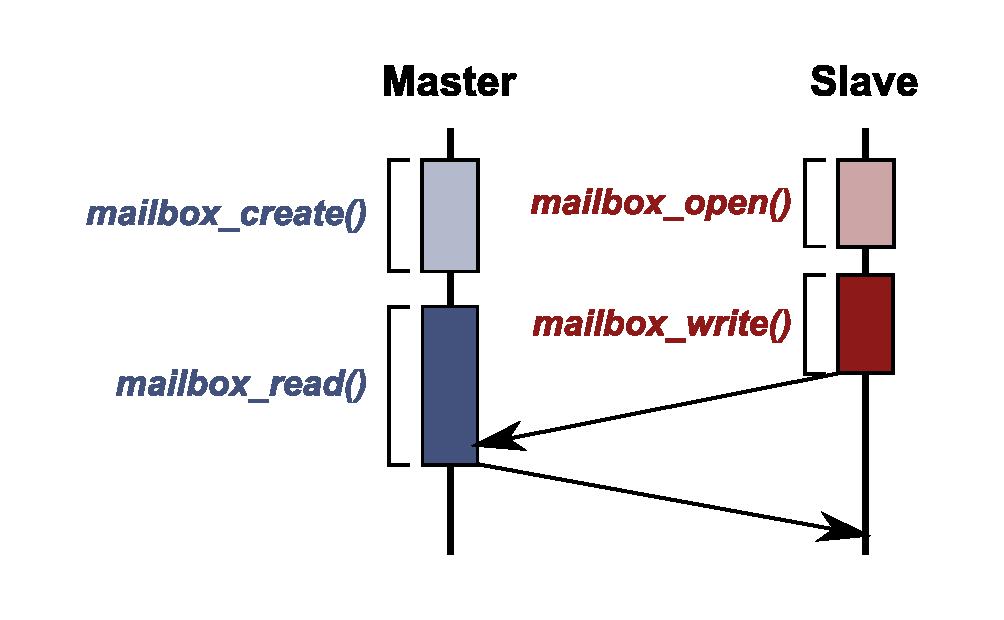
\includegraphics[width=\linewidth]{mailbox-flow.pdf}}%

					\fonte{Developed by the Author.}%
				\end{figure}

				The \textit{Mailbox Abstraction} allows clusters to exchange fixed-size
				messages with each other.
				The message was thought to be a relatively small size, usually a few hundred bytes.
				Similarly, the operation of the \mailbox follows \posix message queue behavior.
				For example, the message can be used to encode small operations and system
				control signals.
				As illustrated in \autoref{fig:conpt_mailbox}, the operation cardinality is N:1,
				where N senders can transfer one message at a time to a receiver queue.
				When the receiver consumes a message, it notifies the sender to ensure
				control of the flow.

			\subsubsubsection*{Portal Abstraction}
			\label{sec.portal-abs}

				\begin{figure}[t]
					\centering%
					\caption{Portal Abstraction Concept: Node 1 create a portal and notify Node 2 to transfer the data.}%
					\label{fig:conpt_portal}%
					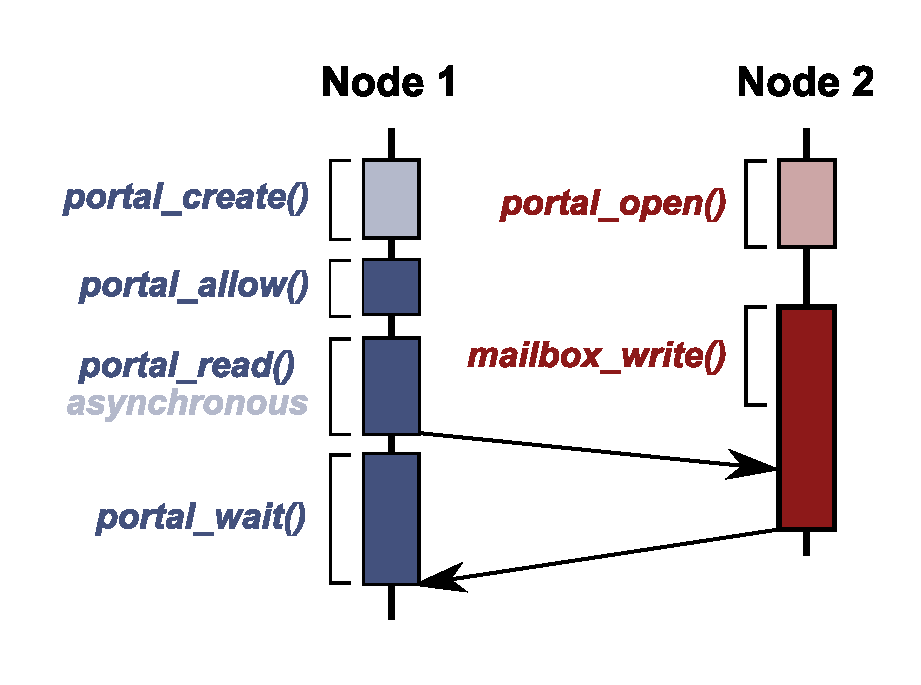
\includegraphics[width=.65\textwidth]{portal.pdf}%
					\fonte{Developed by the Author.}%
				\end{figure}

				Lastly, the \textit{Portal Abstraction} enables two clusters to exchange arbitrary
				amounts of data.
				The conceptual idea of the \portal is similar to that implemented in \posix pipes.
				\autoref{fig:conpt_portal} shows the \portal operation, with cardinality
				1:1, a cluster pair opens a channel to transfer data.
				However, the operation is only allowed in one direction with a flow control mechanism,
				where the receiver cluster warns the sender cluster when it is ready to receive.
		
	\subsection{Communication Services for the Nanvix Microkernel}
	\label{sec.communication-services}
	
		The inter-cluster communication module, described in \autoref{sec.inter-cluster-communication},
		is designed to export a standard and straightforward communication
		primitives to different lightweight manycores.
		These primitives can be used by various types of operating systems
		and applications.
		Thus, the module is flexible enough not to impact the performance
		of the upper layers negatively.
		For this, it does not provide rich management of the exposed abstractions.

		In this scenario, the communication services of Nanvix Microkernel seek
		to provide \ipc between distinct clusters.
		Specifically, these services perform the multiplexing of the hardware
		resources and the verification of the parameters that will be passed
		on the communication primitives.
		Due to the Master-Slave model, the responsibility of protecting,
		manipulating, and configuring \hal resources is of the master core.
		The slave core will request operations through a meta-interface,
		passing the necessary information to the master.

		Considering that the abstractions make up the fundamental elements of
		the construction of more complex services, the Microkernel services
		were responsible for the management and multiplexing of the finite
		resources for the many cores of a cluster.
		In total, there are three communication services in the Nanvix Microkernel,
		each associated with an abstraction of the communication module,
		analogously named \sync, \mailbox, and \portal services.

\chapter{Related Work}
\label{ch.related-works}

The proposal of this work is related to several other research works.
First, some research papers describing state-of-the-art \textit{lightweight} \manycores
processors will be cited. Further, research on different \oss
proposed for such processors will be highlighted.

\section{Lightweight Manycore Processors}
\label{sec.works.manycores}

	In addition to \mppa, many works exemplify the wide variety of architectural
	possibilities of \textit{lightweight} \manycores.
	For instance, Olofsson \etal~\cite{olofsson2014} introduce \epiphany as a
	high-performance energy-efficient \manycore architecture suitable for
	real-time embedded systems.
	The architecture consists of nodes communicating through three 2D mesh \nocs
	with a distributed shared-memory model without coherence protocol.
	Each node has one \risc \cpu, multi-banked local memory, a \dma engine,
	an event monitor and a network interface.
	The three \nocs, named rMesh, cMesh, and xMesh, are independent and scalable.
	They implement a packet-switched model with four duplex links at every node.
	When a node wants to read a remote data, first, it sends a read request over
	the rMesh and wait for a signal to arrive on cMesh.
	On the another hand, the write operation allows the node to continue running
	while data is tranfered through over xMesh.

	On the other hand, for help and facilitate on the \manycore processor design,
	Wallentowitz \etal~\cite{Wallentowitz2013} presents the open-source framework
	\optimsoc which allows build \manycore \soc and simulate them on a computer or
	synthesize them on a \fpga.
	The \pe are \openrisc~\footnote{https://opencores.org/openrisc}
	processor organized in tiles.
	The central architectural element is the LISNoC, a \textit{packet-switched \noc}
	that implements virtual channels to avoid message-dependent deadlocks.
	The LISNoC support various network topologies, depending only on the tiles organization.
	Precisely, a \textit{network adapter} handles the memory transfers between
	tile and the memory and provide hardware means to a message-passing communication
	model among tiles.
	The tiles organization and the network topology also allows handling communication
	in three different ways.
	First, when using distributed memory, communication is performed through the
	message-exchange between the tiles.
	Second, by using a partitioned global address space scattered through the
	local memories of the tiles, the network adapter can perform \mpu-like memory
	address translation hiding the exchange of messages but without providing cache coherence.
	Finally, Wallentowitz \etal study policy of write-through snooping to provide
	a global memory shared among tiles with cache coherence.

	Similarly, Kurth \etal~\cite{Kurth2017} introduce the \hero, which unites an \arm
	host processor with a fully modifiable \riscv \manycore implemented on a \fpga.
	The \pmca uses a multi-cluster design and also relies on multi-banked memory, called \spm.
	The data caches had substituted to a multi-channel \dma engine that copy data
	between a shared L1 \spm and remote \spms or shared main memory.
	Communication to main memory passes through software-managed lightweight \rab.
	The \rab performs the translation of the virtual-to-physical address similar to an \mmu.
	In this way, clusters can share virtual address pointers.
	Besides, exists different designs for the shared instruction caches and
	top-level interconnection such as bus or \noc.

\section{Operating Systems for Lightweight Manycores}
\label{sec.works.os}

	Baumann \etal~\cite{Baumann2009} proposed a new \os architecture for scalable multicore
	systems, called \multikernel.
	In their perspective, the future of the \oss is on embracing the networked nature
	of the machines based on distributed systems ideas.
	Assuming the cores are independent nodes of a network, they build the tradicional
	\os functionalities as fully-featured processes.
	This processes communicate via message-passing and does not share the internal
	structures of the \os.
	The work showed how expensive it is to maintain a state of the \os through
	shared-memory instead of exchanging messages and the subsequent increase of
	the complexity of cache-coherence protocols.
	The \multikernel implementation, named Barelfish, follow three design principles.
	First, \textit{Make all inter-core communication explicit} turns the system
	amenable to human or automated analysis because processes communicate only
	through well-defined interfaces.
	Second, \textit{Make \os structures hardware-neutral} makes the hardware-independent
	code easy to debug, optimize, and facilitates the deploy the \os for new
	processor types, avoiding rework.
	And lastly, \textit{View \os state as replicated instead of shared} improve system
	scalability.

	In Wisniewski~\cite{Wisniewski2014} \etal, the concept of scalability was pushed
	to the extreme, thinking on \hpc.
	The principal motivation is the creation of an \os that simultaneously supports
	programmability, through support \linux \api, and provides a lightweight kernel
	to performance, scalability, and reliability.
	The \os, named \mos, provide as much of the hardware resources as
	possible to the \hpc applications. On the other hand, the Linux kernel
	component acts as a service that provides Linux functionalities.

	In like manner, Kluge \etal~\cite{kluge2014} developed the \moosca.
	With \moosca, they introduce abstractions that are easily composed, called Nodes,
	Channels and, Servers.
	Where Nodes represent execution resources, Channels represent communication
	resources, \eg \noc resources, and lastly, Servers are nodes that provide
	services to client Nodes.
	To meet safety-critical requirements, they partition \manycore and distribute
	replicas of Servers, turning the whole system more predictable.
	However, in order to deal with interferences in shared resources,
	usage policies are introduced to make possible the prediction of system behavior.

	Finally, Nightingale \etal~\cite{nightingale2009} presents the Helios \os to
	simplify the process of writing, deploy, and optimize an application across
	heterogeneous cores.
	They use the microkernel model, naming \textit{satellite kernel}, to export
	a uniform and straightforward set of \os abstractions.
	The most important design decisions were to avoid unnecessary remote communication
	by thinking about the penalty they have in \numa domains.
	Also, request the minimum of hardware primitives so that architectures with many
	constraints can be ported.
	Moreover, request the minimum hardware resources to support architectures with little
	computational power or memory constraints.

\section{Discussion}

	\autoref{sec.works.manycores} exemplifies how \manycore architectures can be
	grouped over a common logic perspective.
	They all have one or more logical units distributed and incorporated on clusters.
	The clusters, interconnected through a network, communicate by message-exchange.
	However, due to the domain for which these processors were designed, they end up
	presenting several differences among them at the hardware level.

	On the other hand, \autoref{sec.works.os} presents studies of \oss that focus on
	mitigating these differences in order to provide greater programmability and portability.
	Nevertheless, they span the entire development spectrum, delivering to end-users
	high-level abstractions for increase productivity.
	In this way, it is possible to notice the extensive rework that all of them had in
	dealing with the closest layer of hardware that, as observed, can be abstracted to
	a common perspective.

	In this context, the proposed \hal deal with the lowest level possible with a focus
	on the aspects that make it challenging to work with \manycores.
	Thus, different \oss and services can be developed and disseminated by various
	architectures that implement this perspective.
	So consequently, the applications that run on top of them.
 \chapter{Proposal}
\label{ch.proposal}

The proposal for this undergraduate dissertation is made up of two main contributions.
The first contribution will be the port of the \textit{Inter-Cluster Communication Module},
described in Section \ref{sec.inter-cluster-communication}, for the \mppa manycore processor.
The second contribution will be the design and implementation of communication services
of a master-slave \os, described in Section \ref{sec.communication-services}, on top of
the communication module.

\section{Inter-Cluster Communication Module}

	Ideally, the \hal implementation should not use any other layer of software to
	deal with the hardware. However, the implementation of \hal in \mppa uses the
	software stack made available by Kalray.
	In order to replace them, a great effort would be necessary, fleeing the proposal
	of this work and the scope of Pedro H. Penna's Ph.D.
	The main reasons for this decision were due to poor documentation and the
	inability to execute kernel mode code freely.

	\begin{figure}[t]
		\centering
		\caption{Software Stack of the \mppa.}

		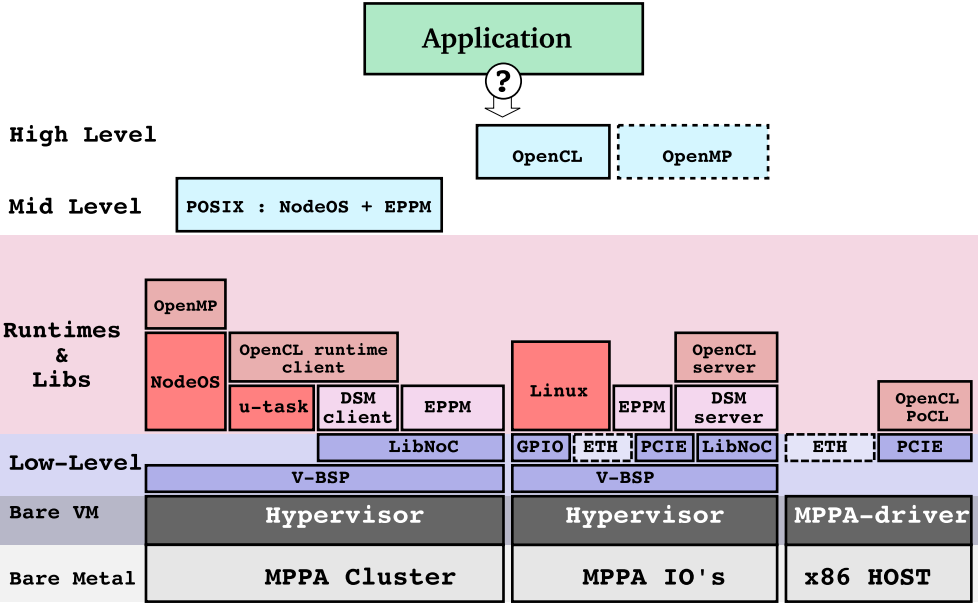
\includegraphics[width=.8\textwidth]{images/software-stack.png}

		\\ \vspace{0.2cm}
		Source: \mppa Processor Documentation.

		\label{fig.software-stack}
	\end{figure}

	Figure \ref{fig.software-stack} shows the software stack present for the \mppa.
	From it, only the \textit{hypervisor} and the \textit{vbsp} library will be used.
	The hypervisor is used to virtualize the hardware by separating it into logical
	parts, e.g., core virtualization, \cnoc virtualization, and \dnoc virtualization.
	It also exports routines to manage, configure, and allow access to virtual resources.
	The vbsp library, in turn, provides primitives for setting interrupts.

	The inter-cluster communication module will use \hal's interfaces and the
	virtualizations of the \cnoc and \dnoc interfaces directly.
	Virtual \noc interfaces export asynchronous calls to acquire read and write
	permission from registers that configure the hardware for a given task.
	For instance, the \dma configuration for asynchronous sending is abstracted by
	$\mu$threads that are configured through global structures provided by the hypervisor.

	\begin{table}[t]
		\caption{Cluster Identification.}

		\begin{tabular}{|l|l|l|}
			\hline
						         & \textbf{Physical ID} & \textbf{Logical ID} \\ \hline
			\textbf{\ccluster}   & 0-15                 & 0-15                \\ \hline
			\textbf{\iocluster0} & 128-131              & 16-19               \\ \hline
			\textbf{\iocluster1} & 192-195              & 20-23               \\ \hline
		\end{tabular}

		\label{tab.cluster-id}
	\end{table}

	Clusters have two identifiers, one physical (physical ID) and the
	other logical (logical ID).
	The physical ID's are the numbers in hardware that identically them
	during the process of routing the data through \noc.
	The logical ID's are numbers associated with the physical ID's so
	that it is possible to identify the clusters outside the \hal.
	Logical ID's primarily serve to disassociate the cluster
	identification from the architecture in which \hal is implemented.
	Table \ref{tab.cluster-id} shows the physical and logical
	identification performed for \mppa.

	\begin{table}[]
		\caption{Partitions of \noc resources by abstraction.}

		\begin{tabular}{l|l|l|l|l|}
			\cline{2-5}
										   & \multicolumn{2}{c|}{\textbf{\cnoc}} & \multicolumn{2}{c|}{\textbf{\dnoc}} \\ \cline{2-5}
										            & \textbf{RX Slot} & \textbf{TX Channel} & \textbf{RX Slot} & \textbf{TX Channel} \\ \hline
			\multicolumn{1}{|l|}{\textbf{\mailbox}} & 0-23             & 0                   & 0-23             & 1-3                 \\ \hline
			\multicolumn{1}{|l|}{\textbf{\portal}}  & 24-47            & 1-2                 & 24-47            & 4-7                 \\ \hline
			\multicolumn{1}{|l|}{\textbf{\sync}}    & 48-71            & 3                   & -                & -                   \\ \hline
		\end{tabular}

		\label{tab.noc-resources}
	\end{table}

	To perform the communication between two clusters, it is necessary that the
	sender knows which resource the receiver will use.
	For this reason, the receive slot range of \cnoc and \dnoc are partitioned
	by abstraction, as can be seen in Table \ref{tab.noc-resources}.
	Within a partition, each slot is associated with a cluster's logical ID.
	On the other hand, the transmitters use sending channels that need to
	be reserved during the entire operation.
	Thus, Table \ref{tab.noc-resources} also shows the partition of the
	sending channels for each abstraction.

	\subsection{Sync}

\begin{figure}[t]
\begin{lstlisting}[
	caption=HAL Sync Interface for Receiver Cluster,
	label=code:sync-receiver,
]
	/* @brief Allocates and configures the receiving side of
	 *        the synchronization point.                     */
	int sync_create(const int *nodes, int nnodes, int type);

	/* @brief Releases and cleans receiver buffer. */
	int sync_unlink(int syncid);

	/* @brief Wait signal on a specific synchronization point. */
	int sync_wait(int syncid);
\end{lstlisting}
\end{figure}

\begin{figure}[t]
\begin{lstlisting}[
	caption=HAL Sync Interface for Sender Cluster,
	label=code:sync-sender,
]
	/*  @brief Allocates and configures the sending side of
	 *  the synchronization point.                          */
	int sync_open(void);

	/* @brief Releases the sender resources on a specific DMA channel. */
	int sync_close(int syncid);

	/* @brief Send signal on a specific synchronization point. */
	int sync_signal(int syncid, const int *nodes, int nnodes, int type);
\end{lstlisting}
\end{figure}

		As described in Section \ref{sec.sync-abs}, the \sync abstraction allows the
		creation of distributed barriers.
		The \sync can be decomposed into two sets of functions, where the
		Code \ref{code:sync-receiver} shows the functions to one clusters
		that will receive signals, and Code \ref{code:sync-sender} shows the
		ones that will send.
		Each set allocates different types of resources.
		Accurately, the receiver must allocate a receive slot of the frame,
		and the transmitter will allocate a transmitter channel of the frame.
		Because of this, 24 synchronization points can be created (\texttt{sync\_create()}),
		and only 1 can be opened (\texttt{sync\_open()}) per cluster.

		Sync Functions implement two different types, depending on who cluster
		should be the master of the synchronization operation.
		Specifically, every synchronization operation is separated into a
		master cluster and one or more slave clusters defined by the
		\texttt{ONE\_TO\_ALL} and \texttt{ALL\_TO\_ONE} constants.
		The master always takes the role "ONE" and the slaves the "ALL" role.
		The following subsections describe the behavior and implementation
		details of each type of synchronization.

			\subsubsection*{\texttt{ONE\_TO\_ALL} Synchronization Type}

				The slave clusters involved in this type of synchronization expect
				a signal sent from the master.
				To do this, each slave will perform the function \texttt{sync\_create()}
				by allocating the resource associated with the master's logical ID.
				After allocating and configuring the resource, the cluster can
				continue to run without worrying about whether the signal was received.
				When the time comes to perform the synchronization, it is enough for
				the slave to run the function.
				Upon receiving the signal, the sync will auto reconfigure the resource
				and free the cluster.

				The cluster master, in turn, must perform the complementary functions.
				That is, first, the master will allocate a sending resource by calling
				the \texttt{sync\_open()} function.
				After that, it should inform the set of clusters that will receive the
				signal on its logical ID.
				Finally, both can release sync resources by calling release functions,
				\texttt{sync\_unlink()} for the slave and \texttt{sync\_close()} to
				the master.

			\subsubsection*{\texttt{ALL\_TO\_ONE} Synchronization Type}

				Analogously to the previous type, the only changes are just on
				the roles in which they are reversed.
				The master must perform the functions of creation, configuration
				of the resources, and waiting for the numerous signals.
				The resource allocated by the master must be the resource
				associated with its logical ID.
				On the other hand, the slaves will perform the functions of
				opening and sending a signal on the master's logical ID.

	\subsection{Mailbox}

\begin{figure}[t]
\begin{lstlisting}[
	caption=HAL Mailbox Interface for Receiver Cluster,
	label=code:mailbox-receiver,
]
	/* @brief Creates a mailbox. */
	int mailbox_create(int nodenum);

	/* @brief Destroys a mailbox. */
	int mailbox_unlink(int mbxid);

	/* @brief Reads data from a mailbox. */
	ssize_t mailbox_read(int mbxid, void * buffer, size_t size);
\end{lstlisting}
\end{figure}

\begin{figure}[t]
\begin{lstlisting}[
	caption=HAL Mailbox Interface for Sender Cluster,
	label=code:mailbox-sender,
]
	/* @brief Opens a mailbox. */
	int mailbox_open(int nodenum);

	/* @brief Closes a mailbox. */
	int mailbox_close(int mbxid);

	/* @brief Writes data to a mailbox. */
	ssize_t mailbox_write(int mbxid, const void * buffer, size_t size);
\end{lstlisting}
\end{figure}

		As explained in Section \ref{sec.mailbox-abs}, the \mailbox abstraction
		allows the exchange of small messages of sizes between clusters similar
		to a \posis message queue.
		The \mailbox is more complex than the previous abstraction because it
		uses both \dnoc and \cnoc resources.
		When executing the function \texttt{mailbox\_create()}, the receiver
		will only use one \dnoc receive slot and configures it with a kernel
		memory space, sufficient to receive 24 messages.
		The messages are composed of the header identifying the sender
		and a body containing the useful message.
		When consuming a message (\texttt{mailbox\_read()}), the receiver
		will copy the message to the user's buffer and send a signal
		to the sender informing him that it can send another message.
		If there is no message in the buffer, the receiver is blocked
		until a message is received.

		On the other hand, the sender will allocate a receive signal slot (\texttt{mailbox\_open()})
		before sending its first message to the receiver.
		If the sender attempts to send a message before the receiver has consumed
		the previous message, the sender will be blocked waiting for the sender's notification.
		In this way, flow control is guaranteed, and the sender will not overwrite
		messages unread by the receiver.
		Sending the message will always be executed asynchronously
		because it will always be necessary to copy the message to
		a kernel buffer that contains the header.
		Thus, the sender will never be blocked waiting for the message to be sent.
		In this configuration, the number of mailbox creations (\texttt{mailbox\_create()})
		within a cluster is limited to 1 because of the \cnoc sending channel.
		On the other hand, the maximum number of opens (\texttt{mailbox\_open()}) is
		4 because of the limitation of the available \dnoc sending channels.

	\subsection{Portal}

\begin{figure}[t]
\begin{lstlisting}[
	caption=HAL Portal Interface for Receiver Cluster,
	label=code:portal-receiver,
]
	/* @brief Creates a portal. */
	int portal_create(int local);

	/* @brief Destroys a portal. */
	int portal_unlink(int portalid);

	/* @brief Allow sender to transfer data. */
	int portal_allow(int portalid, int remote);

	/* @brief Reads data asynchronously from a portal. */
	ssize_t portal_read(int portalid, void * buffer, size_t size);

	/* @brief Waits for an asynchronous operation on a
	 *        portal to complete.                      */
	int portal_wait(int portalid);
\end{lstlisting}
\end{figure}

\begin{figure}[t]
\begin{lstlisting}[
	caption=HAL Portal Interface for Sender Cluster,
	label=code:portal-sender,
]
	/* @brief Opens a portal. */
	int portal_open(int remote);

	/* @brief Closes a portal. */
	int portal_close(int portalid);

	/* @brief Writes data to a portal. */
	ssize_t portal_write(int portalid, const void * buffer, size_t size);

	/* @brief Writes data asynchronously to a portal. */
	int portal_awrite(int portalid, const void * buffer, size_t size);

	/* @brief Waits for an asynchronous operation on a
	 *        portal to complete.                      */
	int portal_wait(int portalid);
\end{lstlisting}
\end{figure}

		Section \ref{sec.portal-abs} showed that the portal abstraction is similar to
		a \posix pipe with flow control.
		So, the \portal analogously follows the ideas implemented
		in the \mailbox with the difference of the option to write,
		that can be synchronously or asynchronously.
		The total number of receive data operations (\texttt{portal\_create()})
		is limited to 2 because of the number of available signal sending channels.
		On the other hand, up to 4 send operations (\texttt{portal\_open()})
		can be performed simultaneously because there are 4 available send
		channels for the \portal.

		Function \texttt{portal\_open()} starts the data send operation.
		In it will be allocated a channel of data sending associated with
		a $\mu$thread.
		Also, a signal receiving slot will be allocated to receive the
		signal that will release the sender to transfer data to the receiver.
		In asynchronous send operation (\texttt{portal\_awrite()}), the cluster
		cannot modify or release the buffer until the operation is completed.
		To ensure that the buffer can use, the cluster must call function \texttt{portal\_wait()}.

		The receiver will allocate a receive slot of the \dnoc and a send
		channel (\texttt{portal\_create()}) to receive data from another cluster.
		After setting up the resources (\texttt{portal\_read()}), the receiver
		can notify a sender (\texttt{portal\_allow()}), enabling it to transfer data.
		For this reason, the read operation is always performed asynchronously.
		After receiving the set amount of data, the receiver can use the buffer securely.

	\section{Communication Services}

		As described in Section \ref{sec.communication-services}, three communication
		services will be developed for the Nanvix Microkernel, named \sync, \mailbox,
		and \portal services.
		Each service will be responsible for protecting, managing, manipulating,
		and multiplexing the resources exposed by the \hal communication module.
		These services must take into account the memory constraints and the
		master-slave model chosen for the Microkernel.

		Management and manipulation operations are similar to all services.
		They will be provided through interfaces that function as wrappers
		for the \hal abstraction functions.
		In the implementation of these interfaces, there will be a mapping
		between low-level identifiers, associated with \hal resources,
		and high-level identifiers, associated with resource protection structures.

		The protection operations are mostly similar.
		For instance, the use of unallocated resources, sanitizing entries,
		checking valid identifiers, non-null pointers, and checking
		for conflicting operations (reading in write-only resources).
		In the meantime, there are exceptional cases in some services
		that must be taken.
		For instance, in the \sync service, a cluster cannot synchronize
		with itself, or there is a repetition of identifiers in the
		stipulated set of clusters.

		Finally, some aspects of services and implementation still need
		to be analyzed and will be better detailed in another version
		of the dissertation.
		For example, what resource multiplexing methods will be used
		and their impacts on the Nanvix Microkernel services.

% \chapter{Experiments}
\label{ch.experiments}

% Neste capítulo
	This chapter evaluates the performance of communication services of
	the Nanvix Microkernel running on the \mppa processor, \ie \mailbox
	and \portal. The impacts of the synchronization mechanism were not
	analyzed because it is a simple service that does not directly
	influence node communication, depending greatly on the workload of
	each cluster. Noteworthy, the \sync was used in all benchmarks to
	synchronize the nodes involved due to the different boot times and
	the distinct node roles. The evaluation is divided into two sections.
	First, Section \autoref{sec.evaluation-methodology} describes the
	micro-benchmarks, their motivations, and the parameters used. Second,
	Section \autoref{sec.results-analysis} unveil and discusses our
	experimental results.

	\section{Evaluation Methodology}
	\label{sec.evaluation-methodology}

		To deliver a comprehensive assessment of the communication service, we
		stimulate the services with usual collective communication configurations.
		These configurations are usually found in distributed systems and present
		in the high-level services exported by Nanvix Multikernel. For instance,
		message exchanging between servers and clients, work distribution, and
		gathering results.

        Micro-benchmarks measure the data volume and communication latency
		through the \ioctl interface. In manycores, the nodes that communicate
		with peripherals are the bridge between the user and applications.
		Therefore, in our experiments, \iocluster plays the master role when a
		communication routine requires a master-slave behavior. \ioclusters also
		manages only one of the available interfaces to simplify communication.
		In all micro-benchmarks, only one \pe was used to request microkernel
		services.

		\subsection{Micro-benchmarks}

			To analyze the performance of the communication services, we
			relied in collective communication patters of \mpi, as well as
			common behaviors between clients and servers. The following
			subsections conceptually introduced each of these routines and
			behaviors.

			\subsubsection{Broadcast}

				\textit{Broadcast} is the most widely used communication pattern
				in \mpi. In this routine, a node sends the same data to
				all existing nodes. This process may be implemented in
				several ways, such as, Flat Tree, Binary Tree, Double Tree,
				and Chain~\cite{mpi-survey}. \autoref{fig:exp-broadcast}
				presents the \textit{Flat Tree} algorithm used in the benchmark.
				The Flat Tree defines that the root node should send data
				to everyone without delegating this function to other nodes.
				This routine can be used to send user inputs to a parallel
				program or to send configuration parameters to all
				nodes~\cite{url:mpitutorial}.

				\begin{figure}[!tb]
					\centering%
					\caption{Collective Communication Routines.}%
					\label{fig:mpi-routines}%

					\subcaptionminipage[fig:exp-broadcast]%
						{.35\linewidth}%
						{Example of \mpi Broadcast.}%
						{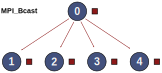
\includegraphics[width=.9\linewidth]{mpi-broadcast.pdf}}%
					\hspace{1cm}%
					\subcaptionminipage[fig:exp-gather]%
						{.35\linewidth}%
						{Example of \mpi Gather}%
						{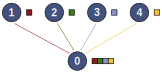
\includegraphics[width=.9\linewidth]{mpi-gather.pdf}}%

					\vspace{0.5cm}%

					\subcaptionminipage[fig:exp-allgather]%
						{.35\linewidth}%
						{Example of \mpi AllGather.}%
						{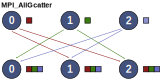
\includegraphics[width=.9\linewidth]{mpi-allgather.pdf}}%
					\hspace{1cm}%
					\subcaptionminipage[fig:exp-ping-pong]%
						{.35\linewidth}%
						{Example of Ping-Pong.}%
						{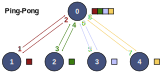
\includegraphics[width=.9\linewidth]{mpi-ping-pong.pdf}}%

					\fonte{Adapted from \citeonline{url:mpitutorial}.}%
				\end{figure}

			\subsubsection{Gather}

				\textit{Gather} is the inverse operation of a broadcast variant
				called scatter. \autoref{fig:exp-gather} illustrates the reverse
				data flow, where this routine gathers the data distributed on a
				single node~\cite{url:mpitutorial}.	Similarly to broadcast, a
				Flat Tree was implemented where all root nodes send their parts
				directly to the root node.

			\subsubsection{AllGather}

				\textit{AllGather} is a routine that does not have a root node,
				illustrated by \autoref{fig:exp-allgather}. As the name suggests,
				the routine performs several Gather operations so that all
				participating nodes end with all pieces of data gathered. Some
				possible algorithms are Ring Algorithm, Recursive Doubling, Gather
				followed by Broadcast Algorithm. The benchmark implements the
				\textit{Bruck Algorithm} where each node will send its data to a
				node with distance $i$ and receive data from a distance $-i$ until
				all nodes contain the complete data.

			\subsubsection{Ping-Pong}

				Ping-Pong is not an \mpi collective communication routine but
				represents communication from a server answering requests from
				client nodes. \autoref{fig:exp-ping-pong} illustrates
				communication by focusing on the master node, where the master
				receives and answers one request at a time.

		\subsection{Experimental Design}
		\label{subsec:experimental-design}

			The parameters that we used for each micro-benchmark are detailed
			in Table~\ref{tab:benchmarks-parameters}.
		% Portal
			The first set of experiments sought to analyze the throughput
			provided by the Portal service. All micro-benchmarks involve 1
			\iocluster and 16 \cclusters, varying the size of the buffer to
			be transmitted from 4~KB to 64~KB. Larger values were not studied
			due to limitation on physical memory size in \cclusters (\ie 2~MB).
			For instance, AllGather requires approximately a total space of
			1~MB ($17$ nodes $\times$ 64~KB).
		% Mailbox
			The second set aimed to analyze the latency of the Mailbox
			service. The micro-benchmarks executed were practically the same
			as the Portal. However, the buffer size to be transmitted became
			constant, 120~Bytes. The variable parameter of the experiments was
			the number of \cclusters involved in the routines.
			Thus, \iocluster is always the master of routines, and the number
			of \ccluster is changed between 1 and 16.

		% Quantas iterações, limitações de memória e desvio padrão
			\mppa has intrinsic characteristics that guarantee low variability
			between runs. Thus, 50 iterations of each benchmark were performed.
			For each experiment, the first ten iterations were discarded to
			eliminate undesired warm-up effects. Finally, all results discussed
			bellow preset a standard error inferior to 1\%.

			\begin{table}[!tb]
				\centering%
				\caption{Micro-benchmark parameters for experiments.}%
				\label{tab:benchmarks-parameters}%

				\begin{tabular}{l|c|c|c|l|}
					\cline{2-5}
															 & \multicolumn{2}{c|}{\textbf{\portal}}   & \multicolumn{2}{c|}{\textbf{\mailbox}} \\ \cline{2-5}
															 & \textbf{Clusters} & \textbf{Data Size}  & \textbf{Clusters} & \textbf{Data Size} \\ \hline
					\multicolumn{1}{|l|}{\textbf{Broadcast}} & 1 IO, 16 CC       & 4, 8, 16, 32, 64 KB & 1 IO, 1 to 16 CC  & 120 B              \\ \hline
					\multicolumn{1}{|l|}{\textbf{Gather}}    & 1 IO, 16 CC       & 4, 8, 16, 32, 64 KB & 1 IO, 1 to 16 CC  & 120 B              \\ \hline
					\multicolumn{1}{|l|}{\textbf{AllGather}} & 1 IO, 16 CC       & 4, 8, 16, 32, 64 KB & 1 IO, 1 to 16 CC  & 120 B              \\ \hline
					\multicolumn{1}{|l|}{\textbf{Ping-Pong}} & 1 IO, 16 CC       & 4, 8, 16, 32, 64 KB & 1 IO, 1 to 16 CC  & 120 B              \\ \hline
				\end{tabular}

				\fonte{Developed by the author.}%
			\end{table}


	\section{Result Analysis}
	\label{sec.results-analysis}

		This is a introduction of the section.

		\subsection{Portal Throughput Analysis}

			\autoref{fig:exp-portal} presents the throughput of the Portal in MB/s
			relative to the different amounts of data transmitted. Results exhibit
			three distinct behaviors in the experiments. First, the Broadcast was
			expected to have the worst transmission rate due to the use of a single
			data transmitter. Since the measurement was done on the receiver side,
			the last slave had to wait for master transmits to all other nodes,
			considerably reducing the transfer rate in the Broadcast. Second, the
			Gather and Ping-Pong routines exhibited similar results, overlapping
			each other on the chart. This similarity is because the master node
			receives multiple requests and handles them serially one by one.
			The master node dictated the data flow in both benchmarks because
			transmission is only performed when allowed by the receiver. Finally,
			the AllGather routine exhibited the best results because of the
			parallelism of communications. Also, each communication pair co-occur,
			and multiple read/write requests not happen at the same time on a node,
			softening the interruption of the master core. In the context of \oss,
			we have subsystems requiring large data transfers, such as file and
			paging systems. In this case, observing the slope of the lines,
			we can infer that the 8~KB and 16~KB sizes favor Portal throughput.
			Overall, the results were as expected, but we believe that solving
			the problem with using DMA accelerators described in
			\autoref{sec.mppa-hardware-resources} could significantly improve
			Portal performance.

			\begin{figure}[!tb]
				\centering%
				\caption{Throughput of the Portal.}%
				\label{fig:exp-portal}%
				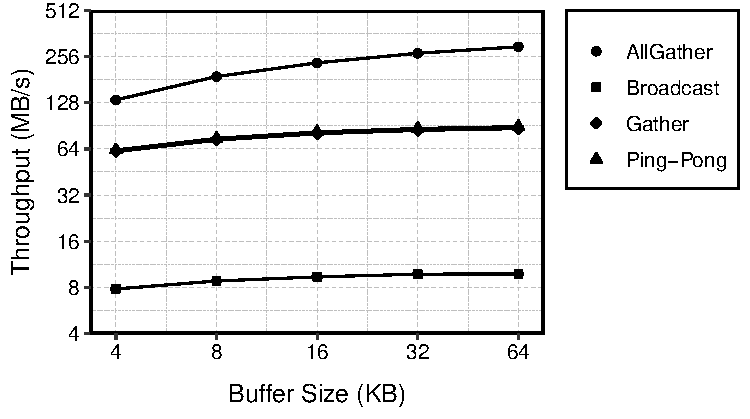
\includegraphics[width=.7\textwidth]{portal-throughput.pdf}%
				\fonte{Develop by the Author.}%
			\end{figure}

		\subsection{Mailbox Latency Analysis}

			\autoref{fig:exp-mailbox} presents the results of the experiments.
			Overall, the routines presented the expected behaviors.
			First, Gather routine, one of the essential routines, had the best
			results because receiving the messages occurs in parallel. Thus,
			the cost after the first message is the overhead of the service
			itself, not the communication. Second, AllGather routine exhibited
			similar behavior to Gather because all clusters send their messages
			before they start reading. Therefore the increase in latency is
			impacted by the transfer operation. The Broadcast routine also
			suffers from the same evil as the on Portal benchmark, where because
			exists only one node sending the messages impacts Mailbox latency.
			Finally, the linear behavior of the Ping-Pong routine is tailored
			by the overhead of sending messages to requesters. It can be noted
			that Ping-Pong has a slightly higher cost than the sum of Gather
			and Broadcast costs, where despite the benefits of receiving
			requests in parallel, the master spends most of his time handling
			requests sequentially.

			\todo[inline]{Sempre que você disser que o comportamento foi
				como o esperado, explicar antes o porque você esperava
					aquele comportamento.}

			\todo[inline]{Novamente, fazer um paralelo qualitativo dos
			resultados com o uso dessas primitivas no sistema. Ping-pong
			evidencia a latencia de comunicacao entre os subsistemas
			do Nanvix com o kernel remoto, mostrando um potencial
			para melhora com DMA pela plataforma. Broadcast, all
			gather e gather evidenciam como algoritmos
			distribuídos de concensus podem ser suportados
			de forma eficiente no multikernel.}

			\begin{figure}[!tb]
				\centering%
				\caption{Latency of the Mailbox.}%
				\label{fig:exp-mailbox}%
				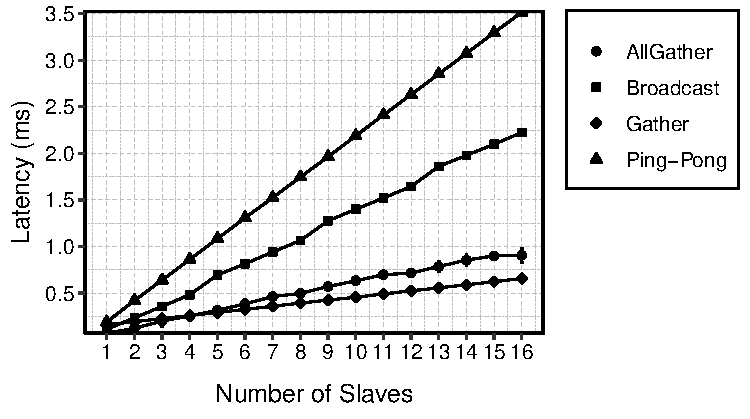
\includegraphics[width=.7\textwidth]{mailbox-latency.pdf}%
				\fonte{Develop by the Author.}%
			\end{figure}

\chapter{Schedule}
\label{ch.schedule}

This chapter presents the schedule for the next activities
planned for the development of the undergraduate dissertation.

\section{Activities}
\label{sec:gantt}

% \begin{figure}[!h]
% 	\caption{Chart Gantt of the Schedule.}

% 	\begin{center}
% 		\begin{ganttchart}[
% 			x unit=0.6cm,
% 			y unit title=0.6cm,
% 			y unit chart=0.6cm,
% 			hgrid,
% 			vgrid={{dotted, dotted, dotted, dotted, dotted, dotted}},
% 			% title label font=\3scriptsize,
% 			title/.append style={fill=gray!30},
% 			title height=1,
% 			bar/.append style={fill=gray!30,rounded corners=2pt},
% 			bar label font=\scriptsize,
% 			group label font=\scriptsize,
% 		]{7}{12}

% 		\gantttitle{\textbf{Meses}}{6} \\
% 		\gantttitle{\textbf{2019}}{6} \\
% 		\gantttitlelist{7,8,9,10,11,12}{1} \\
% 		\ganttbar{1. Writing the Implementation and Experiments.}{7}{9} \\
% 		\ganttbar{2. In-depth Writing of the Proposal.}{9}{10} \\
% 		\ganttbar{3. Presentation of the Undergraduate Dissertation.}{11}{11} \\
% 		\ganttbar{4. Review and Final Submission of the Undergraduate Dissertation.}{12}{12} \\

% 		\end{ganttchart}
% 	\end{center}

% 	\label{chart.gantt}
% \end{figure}

	ANTIGO GANTT shows the planned activities and their durations visually.
	Beginning in July 2019, the final submission is planned for December 2019.
	In detail, the activities are described below:

	\begin{itemize}
		\item \textit{Writing the Implementation and Experiments:}
			Currently, the inter-cluster communication module has the \sync abstraction
			completed and part of the \mailbox abstraction.
			Since the \portal abstraction uses the same low-level mechanisms of the others
			abstractions, its implementation will be facilitated.
			The communication services already have prototypes developed by the author
			for a symmetric \os.
			In this way, the prototypes will need to be modified to use the \hal and
			modified for a master-slave model.
			Finally, micro-benchmarks will be developed to perform an analysis of the
			performance of the implemented services.
		\item \textit{In-depth Writing of the Proposal:}
			During September and October, this activity will be committed to improving
			this draft and detailing the project decisions chose and implementations produced.
			We will also describe the experiments performed and discuss the results obtained.
		\item \textit{Presentation of the Undergraduate Dissertation:}
			November will be dedicated to the development and preparation of the presentation
			of the work and the results achieved.
			So finally, to present the dissertation to the evaluators.
		\item \textit{Review and Final Submission of the Undergraduate Dissertation:}
			Finally, December will be dedicated to the correction of the issues indicated
			by the evaluators and finalized with the final submission of the dissertation.
	\end{itemize}

 \chapter{Conclusions}
\label{ch.conclusions}

Initially, this work presented a historical context of multicore
processors to the nowadays.
By demonstrating the relationship between the growth of the number
of core and energy consumption, it was discussed how academia and
industry began to develop alternatives to alleviate the technological
barriers that have emerged.
However, even new processors that emerge and stand out because of
their performance and power consumption,
they sin in programmability and portability because of their architectural
features, such as hybrid programming model, restrictive memory subsystems,
lack of cache coherence, and heterogeneous configurations.
Part of the difficulty stems from the incompleteness of existing \oss and
runtimes in dealing with severe architectural constraints.

In this work, we present a inter-cluster communication module
designed around the main points in the development of an \os for \textit{lightweight manycores}.
As a basis, we discussed hardware and software aspects of parallel
and distributed architectures.
Different models of \os approaches have been presented that can
use the communication module.
Thus, to provide the basic functionalities for such \oss, three
communication abstractions have been proposed for \hal with the
concern of providing \qos.
Among them is the \sync abstraction to create distributed barriers.
The \mailbox abstraction provides the exchange of small messages
with flow control.
So finally, the \portal abstraction allows the exchange of
arbitrary amounts of data between two clusters.

Another contribution of this work was the communication services
for an operating system based on the microkernel approach.
These services provide for the multiplexing of the resources
exposed by \hal and the verification of the parameters required
for each abstraction.
In general, these services securely export the communication
abstractions to the user, benefiting from the non-competition
of \os internal structures because of the separation of master
and slave responsibilities.
Lastly, the proposal detailed, in general, several aspects of
the implementations.
Because the communication services depend on the \hal communication
module to be developed, the topics associated with
the module have become more detailed and better explored.
However, the next version of the undergraduate dissertation
will clearly and objectively specify both contributions of this work.

% \chapter{Basic Concepts}
\label{ch.basic}

\section{Figure Examples}

Figure.

\begin{figure}[htb]
    
\includegraphics[width=.4\textwidth]{images/ufsc_pb.pdf}
    
    \caption[Short Caption]{
        Long version of caption.
    }
\label{fig.cu}
\end{figure}

\subsection{Sub Figures}
Ref global Figure~\ref{fig.logo} and its subfigures~\ref{sfig.logoA}, \ref{sfig.logoB} and \ref{sfig.logoC}.

\begin{figure}[th]
    \subfloat[]{ 
\includegraphics[width=.2\linewidth]{images/ufsc_pb.pdf} \label{sfig.logoA} }
    \subfloat[]{ 
\includegraphics[width=.2\linewidth]{images/ufsc_pb.pdf} \label{sfig.logoB} }
    
    \subfloat[]{ 
\includegraphics[width=.2\linewidth]{images/ufsc_pb.pdf} \label{sfig.logoC} }
    
    \caption[Short Caption 2]{
        Long version of caption 2.
    }
\label{fig.logo}
\end{figure}

\section{Citations}
\citeonline{Wiegand03} made a nice job.
Citation \cite{Wiegand03}.

\section{Acronym}
See more in wiki\footnote{https://en.wikibooks.org/wiki/LaTeX/Glossary}.
\begin{enumerate}
    \item \gls{dag}.
    \item \glspl{dag}.
    \item \glspl{sram}.
    \item \gls{sram}.
    \item \acrfull{dag}
    \item \acrfullpl{dag}
    \item \test
    \item \test
    \item \tests
\end{enumerate}

\section{Table}

\begin{table}[h]
    \caption[Short Caption.]{
        Table caption here.
    }

    \resizebox{\linewidth}{!}{
        \begin{tabular}{@{}|c|c|c|c|c|c|c|c|c|c|@{}}
            \hline
              & \textbf{June}      & \textbf{July}      & \textbf{August}       & \textbf{September}     & \textbf{October}         & \textbf{November}         & \textbf{December}          & \textbf{January}         & \textbf{February}         \\ \hline
            \textbf{P1} & X & X  &   &   &   &   &   &   &   \\ \hline
            \textbf{P2} &   & X & X &   &   &   &   &   &   \\ \hline
            \textbf{P3} &   &  &  & X &   &   &   &   &   \\ \hline
            \textbf{P4} &   &  &  & X & X  & X  &   &   &   \\ \hline
            \textbf{P5} &   &   &   &   & X & X & X  &   &   \\ \hline
            \textbf{P6} &  &  &  &  &  &  & X & X  &   \\ \hline
            \textbf{P7} &   &   &   &   &   &   &   & X & X \\ \hline
            \textbf{P8} &   &   &   &   &   &   &   &   & X \\ \hline
        \end{tabular}
    }

\label{tab.table}
\end{table}

\section{Equations}
You can use symbols (\primes) from /init/math.

\begin{equation}
    % \displaystyle 
    \jcost(A, B) = + \jlambda \times A \in \integers \in \primes
\label{eq.test}
\end{equation}


\section{Algorithm}

\begin{algorithm}
    \DontPrintSemicolon % Some LaTeX compilers require you to use \dontprintsemicolon instead
    \KwIn{$A=[a_1, a_2, \ldots, a_n]$}
    \KwOut{Max value}
    $max \gets a_1$\;
    \For{$i \gets 2$ \textbf{to} $n$} {
      \If{$a_i > max$} {
        $max \gets a_i$\;
      }
    }
    \Return{$max$}\;
    
    \caption[Short]{
        Max finds the maximum number
    }
    \label{alg.max}
\end{algorithm}

\begin{algorithm}
    \DontPrintSemicolon % Some LaTeX compilers require you to use \dontprintsemicolon instead
    \KwIn{$A=[a_1, a_2, \ldots, a_n]$}
    \KwOut{Max value}
    $max \gets a_1$\;
    \For{$i \gets 2$ \textbf{to} $n$} {
      \If{$a_i > max$} {
        $max \gets a_i$\;
      }
    }
    \Return{$max$}\;
    
    \caption[Short]{
        Max finds the maximum number
    }
    \label{alg.max2}
\end{algorithm}

% =====================================================
% Pós-textuais
% =====================================================
\postextual
\printbibliography

% TODO
%\glossary

% \begin{apendicesenv}

% Imprime uma página indicando o início dos apêndices
\partapendices % this is something of abntex 
% https://github.com/abntex/abntex2/issues/133

\chapter{Quisque libero justo}

Mussum Ipsum, cacilds vidis litro abertis. 
Posuere libero varius. 
Nullam a nisl ut ante blandit hendrerit. Aenean sit amet nisi. 
Interagi no mé, cursus quis, vehicula ac nisi. 
Interessantiss quisso pudia ce receita de bolis, mais bolis eu num gostis. 
Aenean aliquam molestie leo, vitae iaculis nisl. 

\end{apendicesenv}

% \begin{anexosenv}

% Imprime uma página indicando o início dos anexos
\partanexos

\chapter{Morbi ultrices rutrum lorem}

    Mussum Ipsum, cacilds vidis litro abertis. 
    Posuere libero varius. Nullam a nisl ut ante blandit hendrerit. 
    Aenean sit amet nisi. Interagi no mé, cursus quis, vehicula ac nisi. 
    Interessantiss quisso pudia ce receita de bolis, mais bolis eu num gostis. 
    Aenean aliquam molestie leo, vitae iaculis nisl. 
    
\end{anexosenv}


%-----------------
% INDICE REMISSIVO
\phantompart
%\printindex
%-----------------

\end{document}
